\chapter{Grundlagen}
In diesem Kapitel werden einige Grundlagen erläutert, die für den weiteren Verlauf der Arbeit relevant sind.

\section{(Präklinische-) Magnetresonanztomographie}
Magnetresonanztomographie (abgekürzt MRT\footnote{Auch \textit{MRI} (eng. magnetic resonance imaging)}) bezeichnet ein bildgebendes Verfahren, dass den physikalischen Effekt der Kernspinresonanz (englisch: nuclear magnetic resonance (NMR)) nutzt.

Als \textit{Tomografie}\footnote{von altgriechisch tome, Schnitt und graphein, schreiben}-Verfahren ermöglicht es die MRT, dreidimensionale Strukturen als Schnittbilder aufzunehmen und diese zusammengesetzt wieder in 3D darzustellen. Die Schnittbilder geben die innere Struktur eines Objektes dabei so wieder, als wäre das Objekt tatsächlich in der betrachteten Ebene geschnitten. Insbesondere sind die Bilder im Vergleich zu Projektionsverfahren (wie z.B. der klassischen Röntgenaufnahme) über\-lagerungs\-frei.

Im Gegensatz zur \textit{Computertomographie} (CT), einem weiteren sehr verbreitetem Tomographieverfahren, kommt bei einer MRT Untersuchung keine ionisierende Strahlung zum Einsatz.

Die folgenden Abschnitte beschreiben den NMR-Effekt und die weiteren Techniken, die zur Bildentstehung in einem MRT Gerät nötig sind. Im letzten Abschnitt wird auf die Besonderheiten der präklinischen Bildgebung eingegangen.

\subsection{Vom NMR-Effekt zur MRT}
Die Entwicklung der Magnetresonanzbildgebung wurde erst durch die Entdeckung der Kernspinresonanz möglich. Der physikalische Effekt wird auch außerhalb englischsprachiger Länder meist \textit{nuclear magnetic resonance}, kurz NMR, genannt.

1922 zeigten \textsc{Stern}($\ast$1888 $\dag$1969) und \textsc{Gerlach}($\ast$1889 $\dag$1979) im nach ihnen benannten Stern-Gerlach-Experiment die Quantelung von (Eigen-) Drehimpulsen: Silberatome werden aus einem Ofen heraus durch ein inhomogenes Magnetfeld auf eine Glasplatte beschleunigt. Klassisch wäre durch die Ablenkung des Magnetfeldes eine kontinuierliche Intensitäts-Verteilung um $0\degree$ auf der Platte zu erwarten. Stattdessen entstehen durch die quantisierten Spins zwei diskrete Punkte. \cite{Gerlach1922}

1938 konnte die Kernspinresonanz erstmals von \textsc{Isidor Isaac Rabi}($\ast$1898 $\dag$1988) durch eine Erweiterung des Stern-Gerlach-Versuchs nachgewiesen werden: Dazu wird die Anordnung des Stern-Gerlach-Versuchs um ein weiteres inhomogenes Magnetfeld dahinter ergänzt. Dieses ist umgekehrt gepolt und ansonsten identisch zum ersten Feld. Das erste Feld wirkt daher de-fokussierend auf die Atome, das zweite re-fokussierend. Wird ein homogenes Wechsel-Magnetfeld zwischen den beiden inhomogenen Feldern erzeugt, sinkt die gemessene Detektorintensität hinter der Anordnung bei einer bestimmten Frequenz. Bei dieser Frequenz $\omega_0$ wird die Resonanzbedingungen zwischen zwei Übergängen erreicht. $\omega_0$ heißt daher Resonanzfrequenz. Damit ist es möglich, die benötigte Energie zu bestimmen, um ein atomares, magnetisches Moment anzuregen. Für seine Arbeiten erhielt Rabi 1944 den Nobelpreis für Physik. \cite{Rabi1938}

Weitere Pionierarbeit auf dem Gebiet der NMR leisteten der Schweizer Physiker \textsc{Felix Bloch}($\ast$1905 $\dag$1983) und der US-Amerikaner \textsc{Edward Mills Purcell}($\ast$1912 $\dag$1997): Mit unterschiedlichen Versuchsaufbauten entdeckten die Physiker in den 1940er Jahren fast zeitgleich und unabhängig voneinander den NMR-Effekt in Flüssigkeiten bzw. Feststoffen. Bloch und Purcell wurde 1952 gemeinsam der Nobelpreis für Physik verliehen.

\textsc{Paul Lauterbur}($\ast$1929 $\dag$2007) gelang 1973 die erste Aufnahme eines MR-Bildes: Ein dünnes, mit Wasser gefülltes Röhrchen ist in einem \SI{1.4}{\tesla} starken Magnetfeld platziert. Durch Anlegen von, jeweils um \SI{45}{\degree} weiter rotierten, Feldgradienten wurden Projektionen des Transversalmagnetfeldes der Probe erzeugt. Aus diesen konnten dann mit der, aus der Computertomographie bekannten, Methode der Rückprojektion das Originalbild gewonnen werden \cite{LAUTERBUR1973}.

Sowohl das Team um \textsc{Richard R. Ernst}($\ast$1933), als auch \textsc{Peter Mansfield($\ast$1933 $\dag$2017)} verbesserten die, zu der Zeit noch als \textit{Zeugmatography} oder \textit{NMR Imaging} bekannte, Technik durch die Verwendung von eingestrahlten RF-Pulsen und Ausnutzung der, zur damaligen Zeit noch recht neuen, schnellen Fourier Transformation (FFT) zur Rekonstruktion \cite{Kumar1975}, \cite{Mansfield1977}.

Als die erste medizinische MRT-Aufnahme gilt die Darstellung in \autoref{fig:mansfieldFinger}.

\begin{figure}[H]
	\centering
	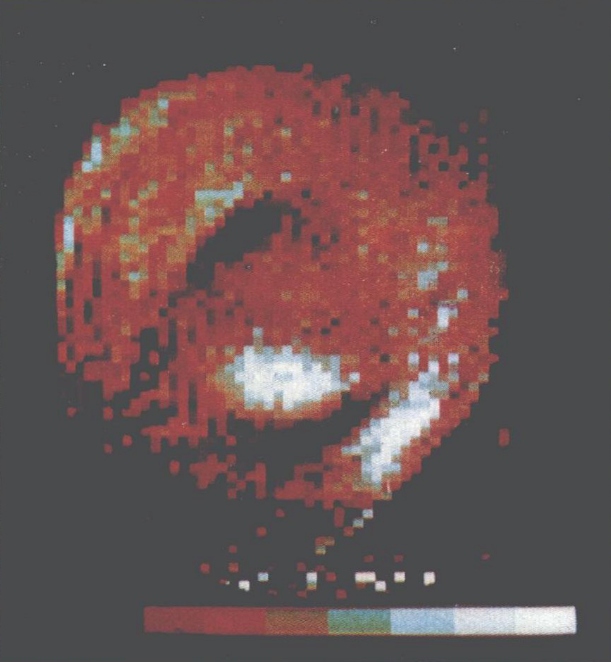
\includegraphics[width=0.5\textwidth]{img/ext/mansfieldFinger.png}
	\caption[Erste MRT Aufnahme von Mansfield]{Erste veröffentlichte MRT Aufnahme (um 1976), Finger mit sichtbarem Knochen, Farbskala kodiert die Signalstärke \cite{Mansfield1977a}}
	\label{fig:mansfieldFinger}
\end{figure}

In \cite{Damadian1971} zeigte der Mediziner \textsc{Raymond Damadian}($\ast$1936) mit Hilfe von NMR Spektren, dass sich gesundes Gewebe und Tumorgewebe in den Relaxationszeiten T1 und T2 (siehe \autoref{sec:theory}) unterscheiden: Krebszellen weisen typisch höhere T1 und T2 Zeiten auf, als das umliegende Gewebe \cite{Damadian1971}. Damit war abzusehen, dass die MRT einen hohen Nutzen in Forschung und Diagnostik haben wird. Danadian meldete 1977 den ersten Ganzkörper-MR-Tomographen zum Patent an.

Paul Lauterbur und Peter Mansfield erhielten 2003 den Nobelpreis für Physiologie oder Medizin.

\subsection{Quantenmechanische Grundlagen}
\label{sec:theory}
\label{sec:nmrTheory}
Atomkerne weisen, ähnlich wie Elektronen, einen Spin auf. Das Spindrehimpuls $\vec{S}$ ergibt sich mit dem Spinoperator $\vec{I}$ und dem reduzierten Planckschen Wirkungsquantum $\hbar$ zu:
\begin{equation}
	\vec{S}=\hbar \vec{I}
\end{equation}

Das magnetische Dipolmoment $\vec{\mu}$ eines Atomkerns ergibt sich aus $\vec{S}$ und dem gyromagnetischem Verhältnis $\gamma$, dass von der Art des Atomkern abhängig ist, zu:
\begin{equation}
	\vec{\mu}=\gamma \vec{S} = \gamma \hbar \vec{I}
\end{equation}

In einem statischen Magnetfeld $\vec{B}=(0,0,B_0)$ ergibt sich in einem makroskopischen Volumen eine Magnetisierung $\vec{M}$:
\begin{equation}
	\vec{M} = \sum \vec{\mu} = (0,0,M_z), \quad \vec{\mu}=(0,0,\mu_z)
\end{equation}

Mit dem angelegten $B$-Feld ergibt sich die potentielle Energie $E$ des magnetischen Dipolmoments zu:
\begin{equation}
	E=-\vec{\mu} \cdot \vec{B} = -\mu_z B_0 = -\gamma S_z B_0 = -\gamma \hbar B_0 |\vec{I}|
\end{equation}

Durch die Quantelung von $\vec{I}$ auf $\vec{I}=(0,0,\pm I_z)$ ergeben sich:
\begin{subequations}
	\begin{align}
	E_1 & = -\gamma \hbar B_0 \frac{1}{2} \\
	E_2 & = +\gamma \hbar B_0 \frac{1}{2}
	\end{align}
\end{subequations}

Damit sind die zwei möglichen Energiezustände $E_1$ und $E_2$ durch
\begin{equation}
	\Delta E = |E_1 - E_2| = \gamma \hbar B_0
\end{equation}
getrennt \cite[S.~ 56]{Nishimura1996}.

Im thermischen Gleichgewicht zeigen $\vec{B}$ und $\vec{M}$ in die selbe Richtung. Ändert sich die Richtung den angelegten Magnetfeldes $\vec{B}$, so tritt Präzession von $\vec{M}$ auf. Aus der Differentialgleichung
\begin{equation}
\label{eq:Mdgl}
	\frac{d\vec{M}}{dt}=\vec{M} \times \gamma \vec{B}
\end{equation}
folgt als Lösung eine Präzession mit einer Kreisfrequenz (auch \textit{Larmorfrequenz} genannt) von
\begin{equation}
	\omega_0=\gamma |\vec{B}|
\end{equation}
bzw. einer Frequenz $f_0$ von
\begin{equation}
	f_0=\frac{\gamma}{2\pi} |\vec{B}| = \frac{\gamma}{2\pi} B_z
\end{equation}

In der MRT werden fast ausschließlich Wasserstoffprotonen für die Visualisierung genutzt. In der MR-Spektroskopie werden neben den \ce{^{1}H}-Kernen noch andere Atomkerne, wie zum Beispiel \ce{^{31}P} oder \ce{^{13}C} genutzt \cite{Andrade2014}. Für die hier erwähnten Atomkerne sind die gyromagnetischen Verhältnisse (geteilt durch $2\pi$) in \autoref{tab:gyroV} angegeben.

\begin{table}[H]
	\centering
	\caption[Auswahl gyromagnetischer Verhältnisse]{Gyromagnetische Verhältnisse einiger Atomkerne \cite{Seidel2015},\cite{Weast1984}}
	\label{tab:gyroV}
	\begin{tabular}{lS}
		\toprule
		\textbf{Kern} & \textbf{$\gamma/2\pi$ (in \SI{}{\mega\hertz\per\tesla})} \\
		\midrule
		\ce{^{1}H} & 42.57056 \\
		\ce{^{31}P} & 17.235 \\
		\ce{^{13}C} & 10.705 \\
		\bottomrule
	\end{tabular}
\end{table}

Wird mit einem Mikrowellensender ein RF-Puls der Energie $E=\gamma \hbar B_0$ so eingestrahlt, dass ein Magnetfeld $B_1$ senkrecht zu $B_0$ entsteht, resultiert daraus
\begin{equation}
	\vec{B}=\vec{B_0}+\vec{B_1}
\end{equation}
wodurch $\vec{M}$ aus dem thermischen Gleichgewicht abgelenkt wird. $\vec{M}$ präzediert daraufhin, wie in \autoref{eq:Mdgl} beschrieben. Je nach Dauer des RF-Pulses kann damit ein beliebiger Winkel $\alpha$ zwischen $\vec{M}$ und $\vec{M}$ im thermischen Gleichgewicht ($\vec{M_{eq}}$) eingestellt werden.
RF-Pulse, die zu einem "Umklappen" von $\vec{M}$ von der $z$-Achse in die $xy$-Ebene führen, werden als \textit{90\degree-Pulse} bezeichnet. \textit{180\degree-Pulse} sind ebenso häufig, zum Beispiel bei Spinecho- oder Inversion-Recovery-Sequenzen (siehe \autoref{sec:SE}), anzutreffen. Anregungspulse für Gradientenecho-Sequenzen (siehe \autoref{sec:GRE}) werden häufig so gewählt, dass die Magnetisierung nicht vollständig in die $xy$-Ebene klappt. Diese Pulse werden dann allgemein als \textit{$\alpha$-Puls}\footnote{In diesem Fall gilt meist: $\alpha<\SI{90}{\degree}$} bezeichnet.

Nach einer Anregung mit einem RF-Puls setzen zwei, voneinander unabhängige Relaxationsphänomene ein \cite{Nishimura1996}:
\begin{itemize}
	\item \textbf{Longitudinale Relaxation:} Mit einer Zeitkonstanten $T1$ wird die Magnetisierung $\vec{M}$ zum thermischen Gleichgewicht $M_{eq}$ zurückkehren. Die Differentialgleichung für die Relaxation der $M_z$-Komponente ist:
	\begin{equation}
		\frac{dM_z}{dt}=-\frac{M_z-M_{z,eq}}{T1}
	\end{equation}
	mit der Lösung:
	\begin{equation}
		M_z=M_{z,eq}+\left(M_z(0)-M_{z,eq}\right) e^{-t/T1}
	\end{equation}
	Unter der Annahme eines 90\degree Anregungspulses bei $t=0$ wird $M_z(0)=0$ und damit:
	\begin{equation}
		M_z=M_{z,eq}\left(1-e^{-t/T1}\right)
	\end{equation}
	\item \textbf{Transversale Relaxation:} Mit einer Zeitkonstanten $T2$ baut sich die transversale Magnetisierung durch Feldinhomogenitäten ab: Durch ein endlich schmales Spektrum der Resonanzfrequenzen in einem makroskopischen Volumen verliert das Spin-Ensemble nach der Anregung seine Phasenkohärenz. Die Relaxation kann durch die Differentialgleichung
	\begin{equation}
		\frac{dM_{xy}}{dt}=-\frac{M_{xy}}{T2}
	\end{equation}
	mit der bekannten Lösung
	\begin{equation}
		M_{xy}=M_{z,eq} e^{-t/T2}
	\end{equation}
	beschrieben werden. Dabei wird angenommen, dass eine 90\degree-Anregung stattgefunden hat, die $M_{z,equ}$ vollständig von der $z$-Achse in die $xy$-Ebene geklappt hat.
\end{itemize}

Präzession und die beiden Relaxationsphänomene können in den \textit{Blochgleichungen} zusammengefasst dargestellt werden.

\subsection{Blochgleichungen}
Die Blochgleichungen (1946 von Felix Bloch in \cite{Bloch1946} vorgestellt) gelten in Flüssigkeiten und eingeschränkt auch in Festkörpern. 
Ohne Relaxation lauten sie (zusammengefasst in vektorieller Schreibweise):
\begin{equation}
\label{eq:bloch1}
	\frac{\vec{M}}{dt} = \gamma \vec{M(t)} \times \vec{B}
\end{equation}
mit:
\begin{with*}
	\vec{M} & Magnetisierung \\
	\vec{B} & externes Magnetfeld (magnetische Flussdichte) \\
	\gamma & gyromagnetisches Verhältnis \\
\end{with*}

Unter Beachtung der Relaxation mit den Zeitkonstanten $T1$ und $T2$ ergibt sich:
\begin{subequations}
	\label{eq:bloch2}
	\begin{align}
	\frac{dM_x(t)}{dt} & = \gamma \left(\vec{M}(t) \times \vec{B}\right) - \frac{M_x(t)}{T2} \\
	\frac{dM_y(t)}{dt} & = \gamma \left(\vec{M}(t) \times \vec{B}\right) - \frac{M_y(t)}{T2} \\
	\frac{dM_z(t)}{dt} & = \gamma \left(\vec{M}(t) \times \vec{B}\right) - \frac{M_z(t)-M_{z,eq}}{T1}
	\end{align}
\end{subequations}
Oder zusammengefasst in vektorieller Schreibweise \cite[S.~61]{Nishimura1996}:
\begin{equation}
\label{eq:bloch3}
	\frac{d\vec{M}(t)}{dt} = \gamma \left(\vec{M}(t) \times \vec{B}\right) - \frac{M_x \vec{e_x} + M_y \vec{e_y}}{T2} - \frac{(M_z-M_{z,eq})\vec{e_z}}{T1}
\end{equation}

Gleichungen \ref{eq:bloch1}, \ref{eq:bloch2} und \ref{eq:bloch3} beschreiben die Spins in einem ruhenden Koordinatensystem (auch "Laborsystem" genannt).
In der Praxis wird das MR Empfangssignal meist mit einem Quadraturmischer mit einer Kreisfrequenz $\omega_T \approx \omega_0$ herunter gemischt. Dies entspricht einer Koordinatentransformation vom ruhenden System $(x,y,z)$ in ein rotierendes Koordinatensystem $(x',y',z')$.
Es ergeben sich die Blochgleichungen im rotierenden System \cite[S.~313]{Doessel2016}:
\begin{subequations}
	\label{eq:blochRot}
	\begin{align}
	\frac{dM'_x}{dt} & = -\frac{1}{T2}M'_x+(\omega_0-\omega_T)M'_y-\omega_F sin(\Psi)M'_z \\
	\frac{dM'_y}{dt} & = -(\omega_0-\omega_T)M'_x-\frac{1}{T2}M'_y+\omega_F cos(\Psi)M'_z \\
	\frac{dM'_z}{dt} & = \omega_F sin(\Psi)M'_x - \omega_F cos(\Psi)M'_y - \frac{1}{T1} (M'_z-M'_{z,eq})
	\end{align}
\end{subequations}
mit:
\begin{with*}
	\omega_0 & lokale Larmorfrequenz\\
	\omega_F = \gamma B_T& Anregungsfrequenz\\
	B_T & Amplitude des anregenden Transversalfeldes $B_1$\\
	\omega_T & Frequenz des Quadraturmischers\\
	\Psi & Phasendifferenz zwischen $B_1$-Feld und Mischer \\
\end{with*}


\subsection{Mit NMR/MRT detektierbare Eigenschaften von Gewebe}
Als bildgebendes Verfahren ist es das Ziel eines Tomographen, Gewebe zu identifizieren und von benachbartem Gewebe zu unterscheiden. Um also zwei Gewebearten in einem MRT Schnittbild unterscheiden zu können, ist es notwendig, dass sich die Gewebe in ihren NMR Eigenschaften hinreichend unterscheiden, so dass dieser Unterschied auch vom Gerät erfasst werden kann. Ein Vergleich einiger Gewebearten zeigt \autoref{tab:gewebe}. Es wird deutlich, dass sich beispielsweise eine Metastase in der Leber mit einer T1 gewichteten MRT Aufnahme gut nachweisen lässt, da sich die T1 Zeiten von gesundem Lebergewebe und der Metastase deutlich unterscheiden.

Mit einem MR-Tomographen werden üblicherweise die folgenden Größen visualisiert:
\begin{itemize}
	\item \textbf{Relaxationszeiten T1 und T2:} Die in \autoref{sec:nmrTheory} erläuterten Relaxationszeiten können durch eine passend gewählte Gewichtung (ortsaufgelöst) gemessen werden
	\item \textbf{Protonendichte PD:} Manchmal auch mit $\rho$ bezeichnet. Eine relative Größe, die darauf schließen lässt, wie viele (mobile) (Wasserstoff-) Protonen ein Gewebevoxel enthält. Die Protonendichte ist zum Beispiel in Knochen viel geringer als in Blut. Sie lässt sich ebenfalls durch eine geeignete Gewichtung messen.  
\end{itemize}

Die chemische Verschiebung kann ebenfalls ortsaufgelöst gemessen werden. Dies wird als \textit{Chemical Shift Imaging (CSI)} bezeichnet \cite{Keevil2006}.

\begin{table}[H]
	\centering
	\caption[MRT relevante Eigenschaften ausgewählter Gewebe]{MRT relevante Eigenschaften von einigen ausgewählten Gewebearten bei einer Feldstärke von \SI{1.5}{\tesla} (in Anlehnung an \cite[S.~16]{Weishaupt2014} und \cite[S.~17]{Reiser2008})}
	\label{tab:gewebe}
	\begin{tabular}{llll}
		\toprule
		\textbf{Gewebe} & \textbf{Protonendichte (in \%)} & \textbf{T1 (in ms)} & \textbf{T2 (in ms)} \\
		\midrule
		Zerebrospinalflüssigkeit & 100 & \textgreater4000 & 2000 \\
		weiße Hirnsubstanz & 70 & 780 & 90 \\
		graue Hirnsubstanz & 85 & 920 & 100 \\
		Fettgewebe & 100 & 260 & 80 \\
		Leber & - & 500 & 43 \\
		Niere & - & 650 & 58 \\
		Metastase & 85 & 1800 & 85 \\
		\bottomrule
	\end{tabular}
\end{table}

\autoref{fig:metastase} zeigt ein T1 gewichtetes, axiales Schnittbild durch eine von Darmkrebs verursachte Metastasierung in der Leber. Das umliegende gesunde Gewebe kann deutlich von den Metastasen abgegrenzt werden.

\begin{figure}[H]
	\centering
	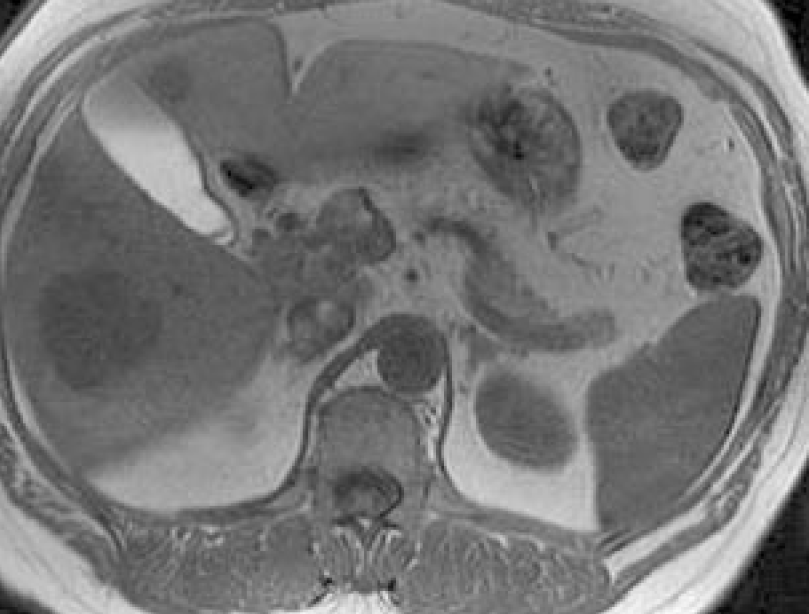
\includegraphics[width=0.5\textwidth]{img/metastase.png}
	\caption[Lebermetastase]{Lebermetastase. Axialer Schnitt, T1 gewichtete spoiled gradient Aufnahme mit Fettunterdrückung, kein Kontrastmittel \cite[S.~872]{Reiser2008}}
	\label{fig:metastase}
\end{figure}

Wie sich die Gewichtung bei einer MRT Aufnahme einstellen lässt, ist in \autoref{sec:gewichtung} gezeigt.

\subsection{Aufbau eines MR-Tomographen}
Der Aufbau eines MR-Tomograpen ist in \autoref{fig:biospecAnot} dargestellt.

\begin{figure}[H]
	\centering
	\resizebox{\textwidth}{!}{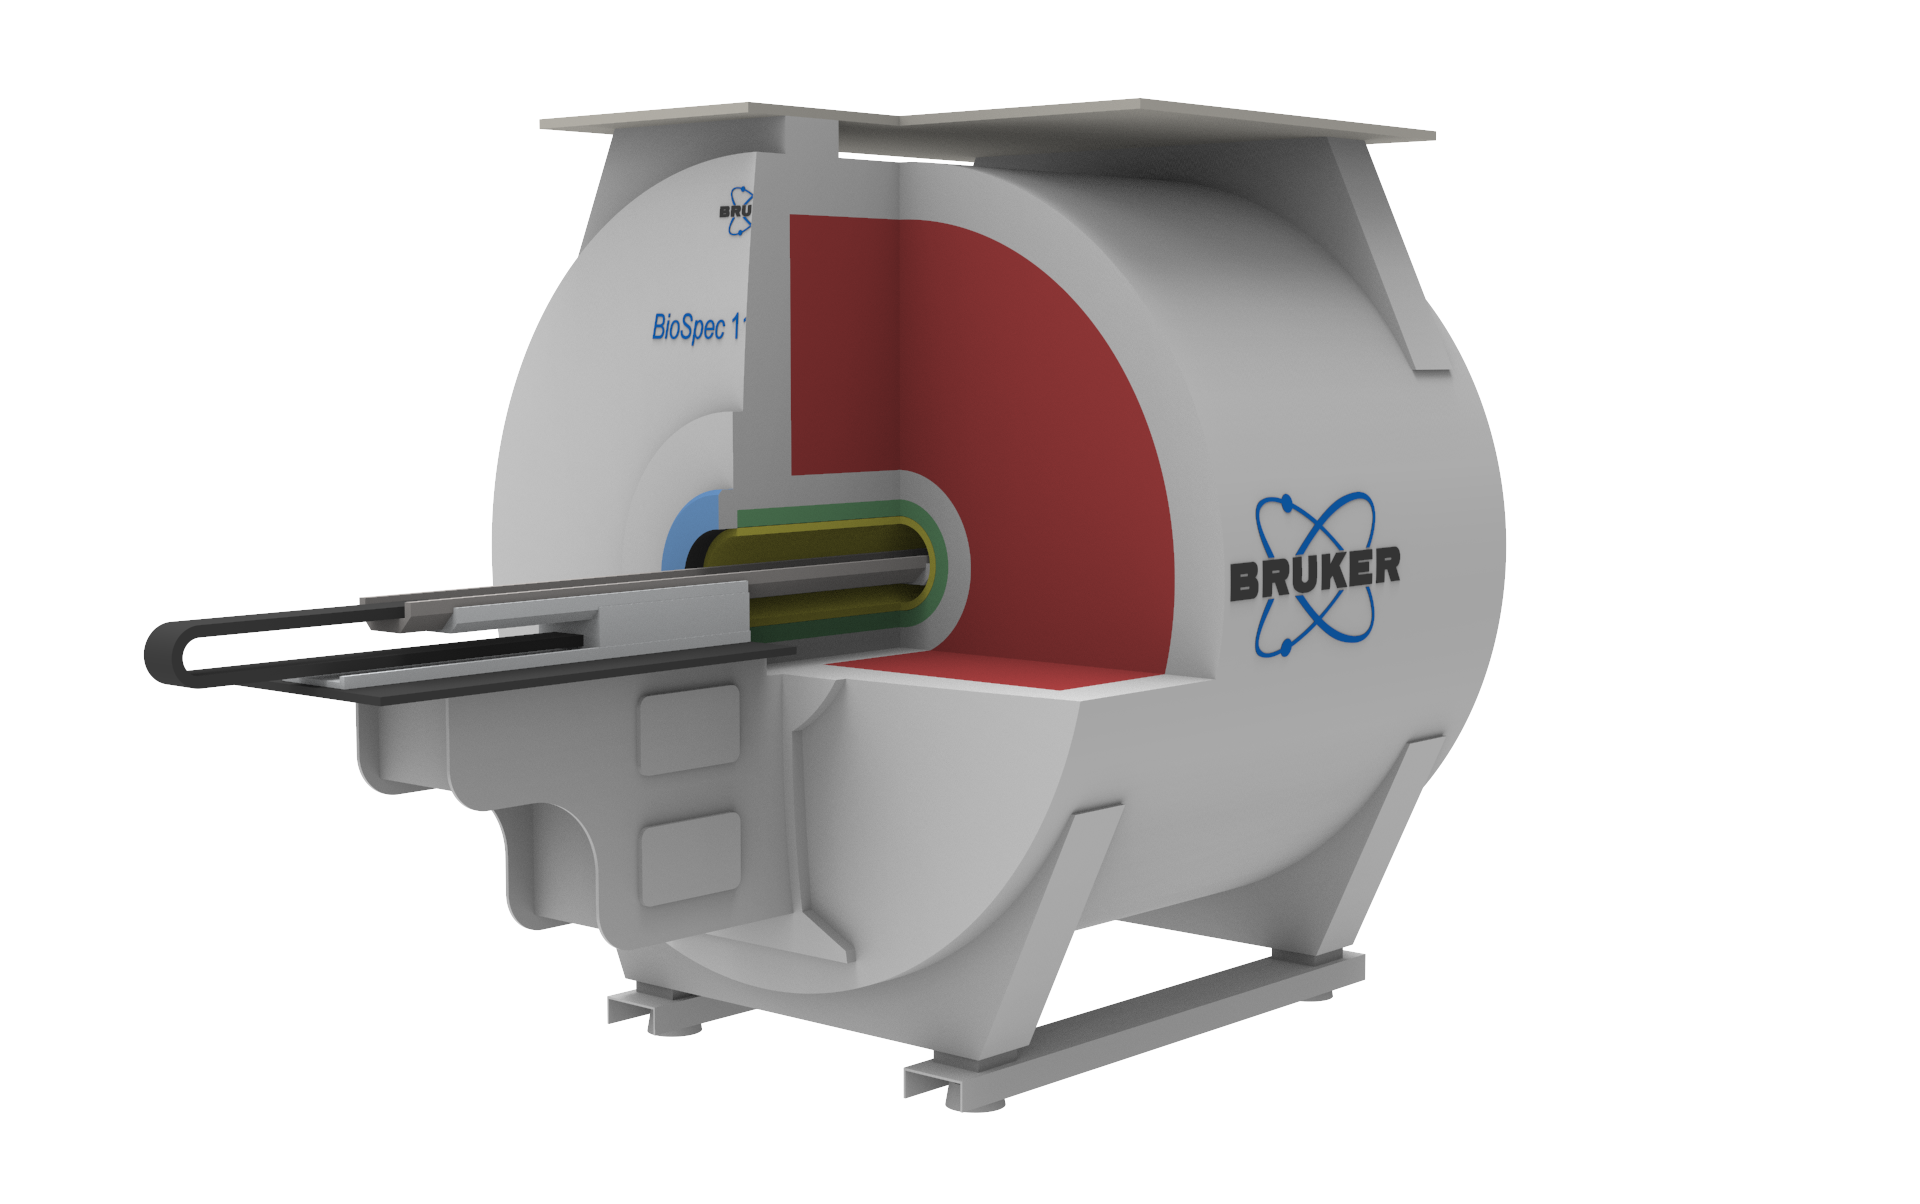
\includegraphics[]{img/biospec.tikz}}
	\caption[Aufbau MR-Tomographen]{Aufbau MRT (ohne Stromversorgung, Steuerungssysteme, Kühlsysteme und Bedienpanel)}
	\label{fig:biospecAnot}
\end{figure}

\subsubsection{Statisches Magnetfeld}
Das statische Magnetfeld, auch $B_0$-Feld genannt, wird durch einen Magneten erzeugt. Dieser muss über eine ausreichend dimensionierte Öffnung verfügen, so dass der zu untersuchende Körper und andere Spulensysteme des Tomographen darin Platz finden. Mit Feldstärken im Bereich von \SI{0.3}{\tesla} (bei klinischen MRT Systemen) bis hin zu \SI{15}{\tesla} im Bereich der präklinischen MRTs ist das $B_0$-Feld verglichen mit dem Erdmagnetfeld\footnote{etwa \SI{50}{\micro\tesla} \cite{Enc1994}} oder einem Kühlschrankmagneten\footnote{etwa \SI{0.1}{\tesla} \cite{LHC2018}} ein sehr starkes Magnetfeld.
Erzeugt wird das $B_0$-Feld entweder mit einem Permanentmagneten oder einem Elektromagneten. 

Auch wenn sich \textit{Permanentmagnet}-Systeme durch ihren einfachen Aufbau und einen kostengünstigen, wartungsfreien Betrieb auszeichnen, sind sie wenig stark verbreitet. Die mit Permanentmagneten erzielbare Feldstärke von etwa einem Tesla ist für die Forderung nach hohem Signal-Rausch-Verhältnissen oft zu gering.

Gewöhnliche Elektromagnete, auch \textit{resistive Elektromagnete} genannt, haben den Nachteil des hohen Stromverbrauchs und der starken Eigenerwärmung. Von Vorteil ist, dass Systeme dieser Bauart bei Nichtbenutzung abgeschaltet werden können. Für sehr hohe Feldstärken sind sie nicht geeignet.

Am weitesten verbreitet sind \textit{supraleitende Elektromagnete}. Nur damit lassen sich wirtschaftlich hohe Feldstärken erreichen. Diese bestehen aus einer supraleitenden Spulenanordnung, welche in einem, mit flüssigem Helium gefülltem, Tank betrieben wird. Da aufgrund der Supraleitung der Spulenwiderstand verschwindet, kann nach einmaligem Aufbau des Spulenstroms die Stromversorgung getrennt werden. Das als Kryostat bezeichnete Kühlsystem verliert durch den sog. \textit{boil-off} kontinuierlich Helium, welches daher regelmäßig wieder aufgefüllt werden muss. Ein Abschalten der Energie- und Kosten-intensiven Kühlung ist nicht möglich. Eine Erwärmung der ganzen Spule, oder Teile davon über die Sprungtemperatur des Spulenmaterials führt zum sog. \textit{Quench}: Die Supraleitung bricht zusammen, das Material wird resistiv und durch die damit verbundene starke Wärmeentwicklung verdampft das gesamte Helium schlagartig. Daher ist es nötig, dass das Kryostat über einen Kamin zur Ableitung des Heliums verfügt. Wenn auch für den Menschen ungiftig, können größere Mengen Helium den Luftsauerstoff verdrängen. Daher muss die Sauerstoffkonzentration in den Aufstellungsräumen überwacht werden.

\paragraph{Shimming}\mbox{}\\
An das statische Magnetfeld werden hohe Anforderungen bezüglich der Feldhomogenität gestellt.
Durch Metalle im Tomographen (Rohre, Schrauben, Befestigungen, etc.) und am Aufstellungsort (z.B. Stahlträger/Metallständerwände), Streufelder anderer Magnete und in die Nähe des Tomographen gebrachte Metalle kommt es zu Inhomogenitäten.
Um diese auszugleichen, wird Shimming (von eng. \textit{shim}, Keil) betrieben. Unterschieden werden passives und aktives Shimming \cite{Lipton2008}:
\begin{itemize}
	\item \textbf{passives Shimming:} Durch gezieltes Einbringen von ferromagnetichen Metallen\footnote{z.B. Eisen oder Nickel} werden Inhomogenitäten statisch korrigiert. Damit können lediglich intrinsische Effekte des MRT-Systems und des Gebäudes ausgeglichen werden.
	\item \textbf{aktives Shimming:} Durch zusätzliche Spulen\footnote{meist in resistiver Ausführung} werden (schwache) Korrektur-Felder erzeugt. Der Vorteil hierbei ist, dass dynamisch korrigiert werden kann: Kurz vor einer MRT Aufnahme kann das aktive Shimming genutzt werden, um Inhomogenitäten  durch die Probe zu mindern.  
\end{itemize}

\subsubsection{Gradientenspulen}
Das Gradientensystem besteht aus mehreren Spulenanordnungen, die dem starken statischen Feld schwächere, zeitlich variable Felder überlagern. Im Gegensatz zum $B_0$-Feld, sind diese Felder \textit{in}homogen. Ihre Feldstärke variiert linear mit dem Ort. Diese lineare Feldänderung wird als Gradient bezeichnet und ist meist in x, y oder z-Richtung ausgeprägt. Da diese Felder schnell umgeschaltet werden müssen, können sie nicht als supraleitende Spulen ausgeprägt werden, sondern sind resistiver Art. Das schnelle Umschalten erfordert leistungsstarke elektrische Verstärker.

\subsubsection{RF Sende- und Empfangsspulen}
Das Hochfrequenzsignal wird über die RF Spulen eingestrahlt. Entweder über die gleiche Spule, oder über separate Empfangsspulen wird das entstehende MR-Signal empfangen.

\subsubsection{Abschirmung}
Zum Schutz des MRT vor externer Störstrahlung und zum Schutz der Umgebung (Menschen und andere Geräte) sind Abschirmungen nötig:
Der Magnet für das statische Magnetfeld erzeugt nicht nur das nutzbare $B_0$-Feld, sondern auch magnetische Streufelder. Diese können passiv, z.B. durch Stahlplatten, oder aktiv durch zusätzliche Spulen abgeschirmt werden.

Von den Gradientenspulen erzeugte Streufelder, welche durch Wirbelströme entstehen, können auf ähnliche Art und Weise unterdrückt werden.

Eine RF-Abschirmung des Raumes, in dem der MR-Tomograph betrieben wird, ist notwendig, damit das MRT Gerät keine Störstrahlung nach Außen emittiert und damit keine externen Störsignale die Bildaufnahme stören können.
Dazu ist es zum Beispiel möglich, den kompletten Raum mit einem Metall auszukleiden, um einen Faradayschen Käfig zu bilden. Kupfer ist dafür gut geeignet, da aufgrund seiner geringen Skin-Tiefe im Megahertz-Bereich eine dünne Folie ausreichend ist. \cite{Weibler1993} Problematisch ist die ausreichende Abschirmung der Eingangstür. Durch Materialverschleiß treten dort besonders häufig RF-Lecks auf.

\subsection{Bildentstehung im MR-Tomographen}
Zur Rekonstruktion eines Körpers in einem MRT müssen die Signale, welche die Empfangsspulen erreichen, so beschaffen sein, dass daraus auf ihren Ursprungsort geschlossen werden kann. Für diese Kodierung werden die Gradientenspulen eingesetzt. Zunächst wird parallel zur $xy$-Ebene eine Schicht im Körper ausgewählt. Dann werden die Pixel in diesem Schichtbild so kodiert, dass ihre Position in $x$- und $y$-Richtung bestimmt ist.

\subsubsection{Selektive Anregung/Schichtwahl}
Zur Auswahl einer Schicht parallel zur z-Ebene wird während der Einstrahlung des HF-Pulses ein Gradient in z-Richtung, $G_z=\frac{\partial B_z}{\partial z}$ eingeschaltet.

Die Amplitudenfunktion $B_T(t)$, mit der das HF-Signal moduliert wird, ist so gewählt, dass eine möglichst scharf begrenzte Schicht in z-Richtung selektiert wird (\autoref{fig:rfForm}).

\begin{figure}[H]
	\centering
	\resizebox{!}{!}{\includegraphics[]{img/rfForm.tikz}}
	\caption[Form des RF-Anregungspulses]{Typische Form des RF-Anregungspulses (nach \cite[S.~326]{Doessel2016})}
	\label{fig:rfForm}
\end{figure}

Daher wird meist
\begin{equation}
	B_T(t)=C \frac{sin(x)}{x}
\end{equation}
als Amplitudenfunktion gewählt (siehe \autoref{fig:rfForm}), da die Fourier-Transformierte der (zeitlich unendlich langen) sinc-Funktion ein Rechteck-Puls ist. Da sich ein unendlich langer sinc-Puls nicht realisieren lässt, sind perfekt scharfe Schichtselektionen und beliebig dünne Schichten nicht möglich.

\subsubsection{Phasenkodierung}
Zur Lokalisierung in der $xy$-Ebene wird zunächst ein Phasenkodiergradient (z.B. $\vec{G_y}$ in $y$-Richtung) angelegt. Dieser wird nur kurz für eine konstante Zeit $T_y$, aber mit variabler Amplitude $G_y$ eingeschaltet. Dadurch wird die Präzessionsfrequenz für alle Spins entlang der $y$-Achse kurzzeitig geändert. Nach Abschalten von $\vec{G_y}$ präzedieren alle Spins wieder mit $\omega_0$, aber mit unterschiedlicher Phase. Die nun vorhandene örtliche lineare Zunahme der Phase entspricht einer Ortsfrequenz. Je nach Amplitude des Phasenkodiergradienten wird eine andere Ortsfrequenz in $y$-Richtung eingestellt. Je nachdem, ob die gerade eingestellte Amplitude (und damit Ortsfrequenz) zu einer in $y$-Richtung vorhandenen Ortsfrequenz passt, entsteht ein mehr oder weniger großes MR-Empfangssignal \cite{Bushong2014}, \cite{Edelstein1980}.

\subsubsection{Frequenzkodierung}
Durch den Phasenkodiergradient werden Ortsfrequenzen in $y$-Richtung kodiert. Um ein vollständiges, zweidimensionales Schichtbild zu erhalten, ist noch eine Kodierung in $x$-Richtung nötig. Dazu wird der Frequenzkodiergradient $\vec{G_x}$ (manchmal auch "read out"-Gradient genannt) verwendet. Dieser Gradient wird während des gesamten Auslesevorgangs angelegt. Statt wie bei dem Phasenkodiergradienten nur eine bestimmte Ortsfrequenz pro Auslesevorgang (und damit pro eingestellter Amplitude von $\vec{G_y}$) zu messen, werden während dem Auslesen durch den dauerhaft eingeschalteten $\vec{G_x}$-Gradienten alle Ortsfrequenzen in $x$-Richtung gemessen \cite{Bushong2014}.

\subsubsection{Der k-Raum}
Für den Phasenkodiergradienten und den Frequenzkodiergradienten können die Abkürzungen
\begin{subequations}
	\label{eq:kSpaceEq}
	\begin{align}
	k_x & = \gamma G_x t \\
	k_y & = \gamma G_y T_y 
	\end{align}
\end{subequations}
eingeführt werden\cite[S.~333]{Doessel2016}, da für die Ortsfrequenzen nicht relevant ist, ob sie durch eine Phasen- oder Frequenzkodierung gemessen werden. Die von den Variablen $k_x$ und $k_y$ aufgespannte Ebene wird als \textit{k-Raum} bezeichnet (\autoref{fig:kSpace}).

\begin{figure}[H]
	\centering
	\resizebox{!}{!}{\includegraphics[width=0.4\textwidth]{img/kSpace.tikz}}
	\caption[k-Raum]{k-Raum, drei verschiedene Amplituden $G_y$ des Phasenkodiergradienten sind dargestellt, die jeweils eine andere Zeile des k-Raums selektieren}
	\label{fig:kSpace}
\end{figure} 

Die verschiedenen MRT-Pulssequenzen fahren mit den Gradientenspulen Trajektorien in k-Raum ab, um diesen abzutasten.

\subsubsection{k-Raum Trajektorien}
Die k-Raum Trajektorie in einer zuvor selektierten Schicht ist eine zweidimensionale Parameterkurve mit der Zeit als Parameter:
\begin{equation}
\vec{s_k}(t)=\begin{pmatrix}k_x(t) \\ k_y(t)\end{pmatrix}
\end{equation}

Die Länge einer Trajektorie $l$ zwischen der Zeit $t_0$ und $t_1$ ergibt sich aus dem Wegintegral
\begin{equation}
l=\Delta s = \int_{t_0}^{t_1} \vec{s_k}(t) ds.
\end{equation}

Eine kartesische oder radiale Abtastung (siehe \autoref{fig:kart} bzw. \autoref{fig:rad}) führt zu relativ kurzen Trajektorienlängen $l$, da die Akquisition für jeden "Pfeil" neu startet.

\begin{figure}[H]
	\centering
	\subcaptionbox{kartesisch\label{fig:kart}}{\includegraphics[width=0.3\textwidth]{img/kTrajcart.tikz}}
	\hfill
	\subcaptionbox{radial\label{fig:rad}}{\includegraphics[width=0.3\textwidth]{img/kTrajRad.tikz}}
	\hfill
	\subcaptionbox{Spiral}{\includegraphics[width=0.3\textwidth]{img/kTrajSpiral.tikz}}
	\caption[k-Raum Trajektorien]{Auswahl an typischen Trajektorien zur Aufnahme des k-Raums bei "traditionellen" Sequenzen}
	\label{fig:trajClassic}
\end{figure}

Schnelle Pulssequenzen, wie die Echo-Planar-Sequenz weisen große Trajektorienlängen $l$ auf (\autoref{fig:trajEPI}).

\begin{figure}[H]
	\centering
	\resizebox{!}{!}{\includegraphics[width=0.3\textwidth]{img/kTrajEPI.tikz}}
	\caption[Echoplanar Sequenz]{EPI Trajektorie}
	\label{fig:trajEPI}
\end{figure} 

\subsection{MRT Pulssequenzen}
Die zeitliche Abfolge der Gradientenfelder (Schichtwahl, Phasenkodierung und Frequenzkodierung) und der Hochfrequenz-Anregungssignale wird als MRT Pulssequenz bezeichnet.
Drei wichtige, so genannte Basispulssequenzen sind \cite[S. 999]{Weishaupt2014}:
\begin{itemize}
	\item \textbf{SE}: Spinecho-Sequenz
	\item \textbf{IR}: Inversion-Recovery-Sequenz
	\item \textbf{GRE}: Gradientenecho-Sequenz
\end{itemize}

Darüber hinaus gibt es heute zahlreiche weitere Sequenzen, die zum Beispiel für spezielle Aufnahme-Modi, wie die Diffusionsbildgebung, nötig sind oder die Aufnahmezeit stark verkürzen. Zwei Beispiele für die "schnellen" Sequenzen sind \textit{Turbo-Spinecho} und \textit{Echo Planar Imaging}.


\subsubsection{Spinecho-Sequenz}
\label{sec:SE}
Bei der Spinecho-Sequenz, abgekürzt mit \textit{SE}, erfolgt zunächst eine Anregung der Schicht mit einem 90\degree-RF-Puls, der die Spins in die XY-Ebene klappt. Durch statische Feldinhomogenitäten zerfällt die Magnetisierung nicht mit T2, sondern mit T2*. Da die Spins auseinanderlaufen, wird dieser Prozess als Dephasierung bezeichnet. Nach der Hälfte der Echozeit ($TE/2$) wird ein 180\degree-RF-Puls eingestrahlt. Dieser klappt das Spin-Ensemble um 180\degree. Die Spins laufen daraufhin nach der Zeit $2(TE/2) = TE$ wieder zusammen; es kommt zur Rephasierung. Das dabei entstehende Empfangssignal wird \textit{Echo} genannt (\autoref{fig:SE}).

Nach der Repetitionszeit $TR$ wird die Sequenz wiederholt. Durch Variation des Phasenkodiergradienten $G_{ph}$ wird bei jeder Wiederholung eine andere Zeile des k-Raums ausgewählt, die dann mit dem Frequenzkodiergradienten $G_f$ pixelweise ausgelesen wird.


Die SE-Sequenz hat den Vorteil, dass statische Feldinhomogenitäten vollständig ausgeglichen werden. Durch die einstellbaren Zeiten $TE$ und $TR$ kann eine T1, T2 oder PD gewichtete Aufnahme erzeugt werden.
Der sehr guten Bildqualität steht die lange Aufnahmezeit gegenüber.

\begin{figure}[H]
	\centering
	\resizebox{!}{!}{\includegraphics[]{img/SE.tikz}}
	\caption[Spinecho-Sequenz]{Zeitverlauf der Signale im MRT bei einer Spinecho-Sequenz}
	\label{fig:SE}
\end{figure}

\subsubsection{Inversion-Recovery-Sequenz}
\label{sec:IR}
Eine Variation der Spinecho-Sequenz ist die Inversion-Recovery-Sequenz, kurz IR-Sequenz. Dabei wird vor dem 90\degree-RF-Anregungspuls ein 180\degree-RF-Puls eingestrahlt. Die Zeit zwischen dem 180\degree-RF-Puls (dem sog. Inversionspuls) und dem Anregungspuls wird als Inversionszeit $TI$ (time of inversion) bezeichnet. Durch die einstellbare Inversionszeit kann das Signal einiger Gewebetypen unterdrückt werden oder es können stark T1 gewichtete Bilder erzeugt werden (\autoref{fig:IR}).

\begin{figure}[H]
	\centering
	\resizebox{!}{!}{\includegraphics[]{img/IRE.tikz}}
	\caption[Inversion-Recovery-Sequenz]{Zeitverlauf der Signale im MRT bei einer Inversion-Recovery-Sequenz}
	\label{fig:IR}
\end{figure}

Besonders in der klinischen Diagnostik relevant sind die, auf der IR-Sequenz basierenden, Pulssequenzen \textit{STIR (Short TI Inversion Recovery)} und \textit{FLAIR (Fluid Attenuated Inversion Recovery)}.
STIR nutzt kurze Inversionszeiten, um Fettgewebe in der Aufnahme auszublenden. Da die Selektion über die $T1$-Zeit erfolgt, werden auch andere Gewebe mit Fett-ähnlichen $T1$-Zeiten abgeschwächt\cite{Bydder1985}.
FLAIR Sequenzen werden zur Unterdrückung von Flüssigkeiten, wie zum Beispiel der Zerebrospinalflüssigkeit eingesetzt. Je nachdem, ob das resultierende Bild $T1$ oder $T2$ gewichtet ist, wird zwischen \textit{T1-FLAIR} (vgl. \cite{Melhem1997}) und \textit{T2-FLAIR} (vgl. \cite{Hajnal1992}) unterschieden\cite{Bakshi2001}.

\subsubsection{Gradientenecho-Sequenz}
\label{sec:GRE}
Bei der Gradientenecho-Sequenz (GRE) wird kein 180\degree-RF-Puls zur Erzeugung eines Echos, sondern ein Polaritätswechsel des Frequenzkodiergradientens genutzt. Dadurch, dass der 180\degree-Puls eingespart werden kann, sind viel kürzere Repetitionszeiten $TR$ möglich. Da bei einer kleinen Repetitionszeit auch nur wenig Zeit für eine vollständige $T1$-Relaxation zur Verfügung steht, werden häufig Anregungswinkel von $\alpha<90\degree$ verwendet (\autoref{fig:GRE}).

Durch die kleinen $TR$-Zeiten ist es möglich, dass beim Auslesen noch ein Restsignal von der vorherigen Anregung vorhanden ist. Da sich dadurch der $T1$ Kontrast verschlechtert, wird das Restsignal häufig durch eine gezielte Dephasierung der Spins zerstört. Dies wird als \textit{Spoiling} bezeichnet. Pulssequenzen, die Spoiling einsetzen heißen zum Beispiel \textit{FLASH} ("fast low angle shot", Bezeichnung von Siemens) oder allgemeiner \textit{SPGR} ("spoiled gradient").

Eine andere Strategie ist es, die transversale Magnetisierung bewusst aufrecht zu erhalten und diese für mehrere Echos zu nutzen. Die entsprechenden Pulssequenzen und ihre Weiterentwicklungen heißen \textit{GRASS} bzw. \textit{FIESTA} bei GE oder \textit{FISP} bzw. \textit{TrueFISP} bei Siemens.

\begin{figure}[H]
	\centering
	\resizebox{!}{!}{\includegraphics[]{img/GRE.tikz}}
	\caption[Gradientenecho-Sequenz]{Zeitverlauf der Signale im MRT bei einer (klassischen) Gradientenecho-Sequenz ohne Spoiling}
	\label{fig:GRE}
\end{figure}

\subsubsection{Turbo-Spinecho-Sequenz}
Eine modifizierte, schnellere Variante der Spinecho-Sequenz ist die Turbo-Spinecho-Sequenz. Je nach Hersteller des Tomographens wird sie auch als FSE (Fast Spin Echo, z.B. von GE verwendet) oder RARE (Rapid Acquisition with Refocused Echoes, z.B. von Bruker verwendet) bezeichnet.

\subsubsection{Echoplanar-Sequenz}
Echoplanar-Sequenzen, abgekürzt EPI (von Echo planar imaging), ermöglichen sehr kurze Aufnahmezeiten, da der gesamte k-Raum nach nur einem RF-Anregungspuls gefüllt wird. Heute verbreitet ist die sog. blipped EPI-Sequenz. Bei dieser wird der Phasenkodiergradient im Gegensatz zu der 1977 von Mansfield vorgestellten EPI Variante nicht konstant eingeschaltet, sondern mit kleinen Impulsen (eng. blips) geschaltet (vgl. \cite[S.~299]{Bushong2014}).

\begin{figure}[H]
	\centering
	\resizebox{!}{!}{\includegraphics[]{img/EPI.tikz}}
	\caption[Echoplanar Sequenz]{Zeitverlauf der Signale im MRT bei einer (blipped) EPI-Sequenz}
	\label{fig:EPIseq}
\end{figure}



\subsection{Bildgewichtungen bei Spinecho-Sequenzen}
\label{sec:gewichtung}
In diesem Abschnitt sei exemplarisch anhand der Spinecho-Sequenz gezeigt, wie durch Variation der Aufnahmeparameter eine T1-, T2-, bzw. PD-Gewichtung erzielt werden kann.

Nach \cite{Bushberg2011} gilt bei einem Schichtbild, das mit einer Spinecho-Sequenz aufgenommen wird, für die Pixelintensität (mit $\rho=PD$):
\begin{equation}
\label{eq:SEintensity}
	I \sim \rho \left(1-e^{-\frac{TR}{T1}}\right) e^{\frac{TE}{T2}}
\end{equation}

In \autoref{eq:SEintensity} sind die Parameter $\rho$, $T1$ und $T2$ vom Gewebe in dem betrachteten Pixel abhängig. Die Echozeit $TE$ und die Repetitionszeit $TR$ sind freie Parameter der Pulssequenz.

Für die Verhältnisse $\frac{TR}{T1}$ und $\frac{TE}{T2}$ können vier Fälle unterschieden werden:

\begin{enumerate}
	\item \textbf{$TR/T1\ll1$ und $TE/T2\ll1$}: T1-Gewichtung
	\item \textbf{$TR/T1\gg1$ und $TE/T2\gg1$}: T2-Gewichtung
	\item \textbf{$TR/T1\gg1$ und $TE/T2\ll1$}: PD-Gewichtung
	\item (\textbf{$TR/T1\ll1$ und $TE/T2\gg1$}: Einfluss von sowohl T1 und T2, praktisch keine Bedeutung)
\end{enumerate}
Die Zeitverläufe der longitudinalen und transversalen Magnetisierung für die Fälle 1), 2) und 3) ist in \autoref{fig:Bildgewichtungen} dargestellt. Aus der Abbildung kann zum Beispiel abgelesen werden, dass sich mit einer T1-Gewichtung ein besserer Bildkontrast zwischen grauer und weißer Hirnmasse erreichen lässt, als mit einer PD gewichteten Aufnahme.

\begin{figure}[H]
	\centering
	\subcaptionbox{T1-Gewichtung}{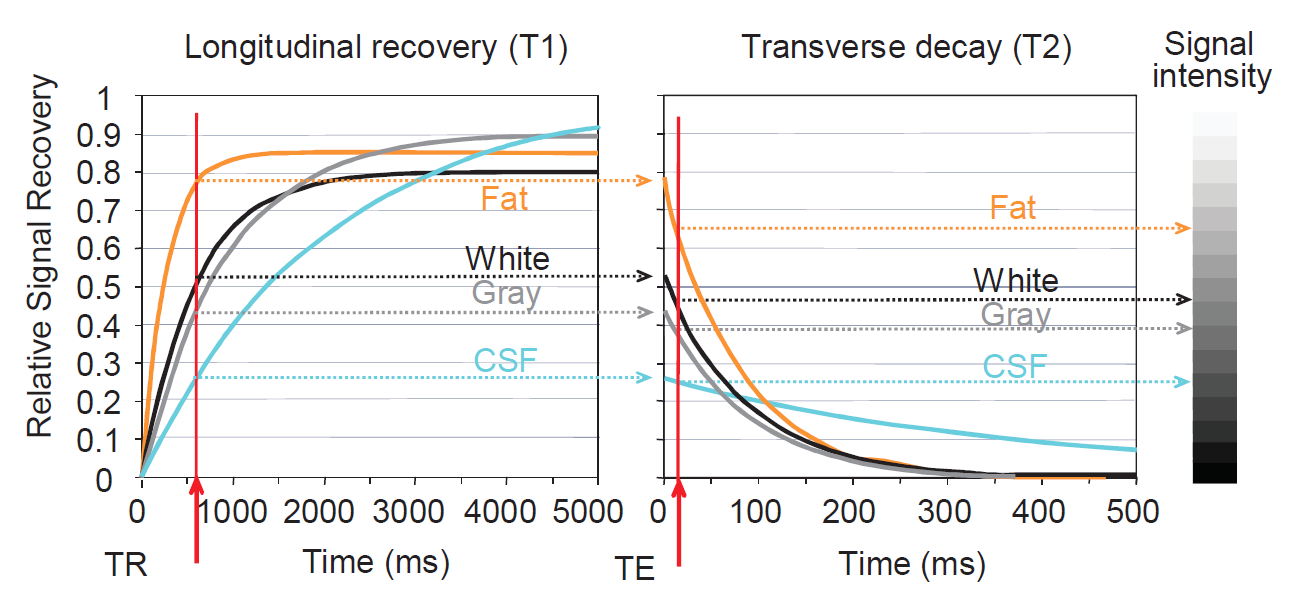
\includegraphics[width=0.8\textwidth]{img/ext/T1W.png}}
	\\
	\subcaptionbox{T2-Gewichtung}{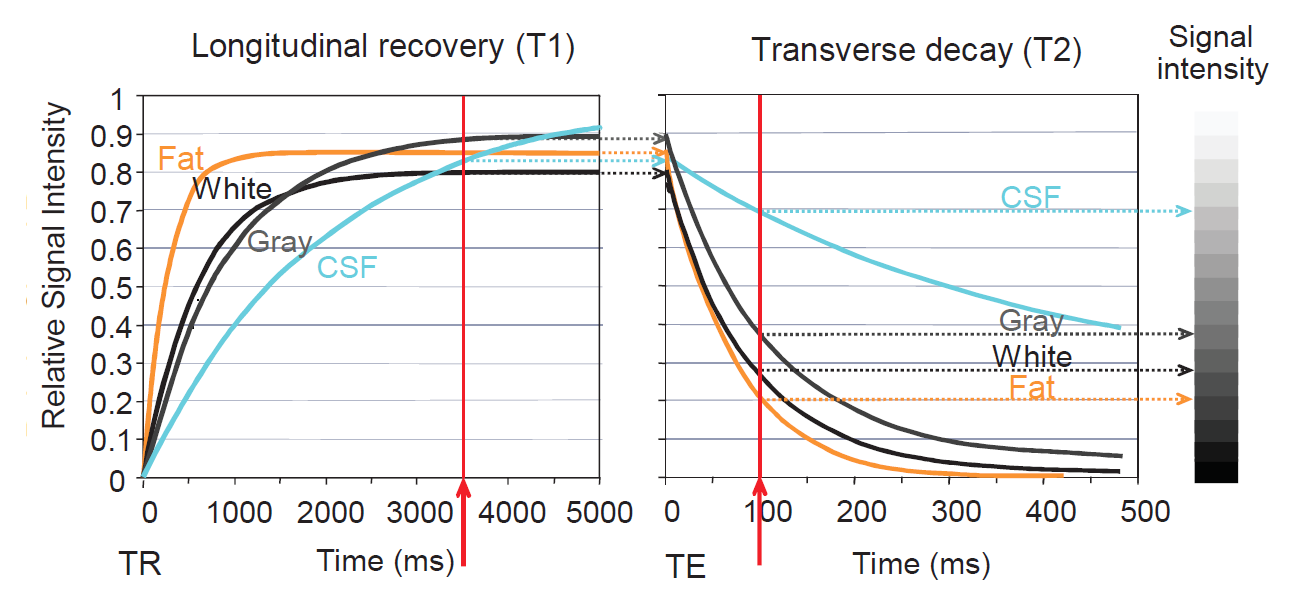
\includegraphics[width=0.8\textwidth]{img/ext/T2W.png}}
	\\
	\subcaptionbox{PD-Gewichtung}{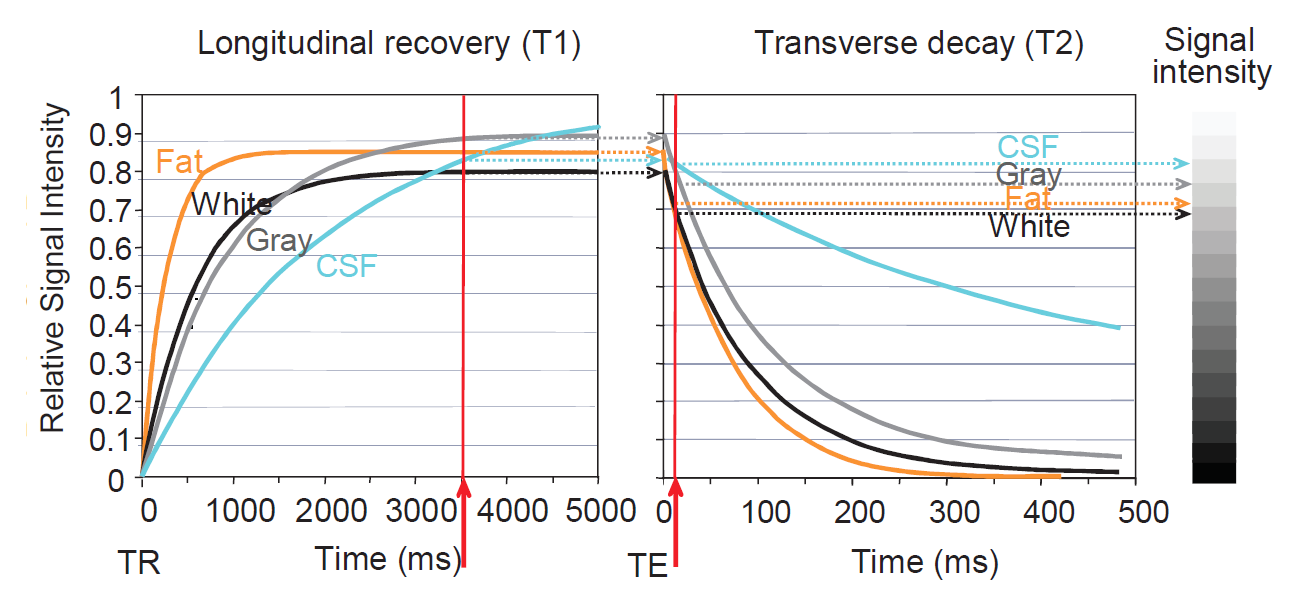
\includegraphics[width=0.8\textwidth]{img/ext/PDW.png}}
	\caption[Bildgewichtung bei Spinecho-Sequenzen]{Wahl der Echozeit $TE$ und Repetitionszeit $TR$ zur Beeinflussung der Bildgewichtung bei Spinecho-Sequenzen (Fat: Fett, Gray: graue Hirnmasse, White: weiße Hirnmasse, CSF: Cerebrospinal fluid (Gehirn-Rückenmarks-Flüssigkeit)) \cite[S.~424ff]{Bushberg2011}}
	\label{fig:Bildgewichtungen}
\end{figure}

\autoref{fig:BildgewichtungenBsp} zeigt drei Schnittbilder identischer Lage durch ein menschliches Gehirn. Durch die Wahl der in den Bildunterschriften angegebenen Echo- und Repetitionszeiten ergibt sich jeweils eine T1-, T2-, bzw. PD-Gewichtung. 

\begin{figure}[H]
	\centering
	\subcaptionbox[T1]{T1 gewichtete Aufname ($TR=\SI{500}{\milli\second}$, $TE=\SI{8}{\milli\second}$)}{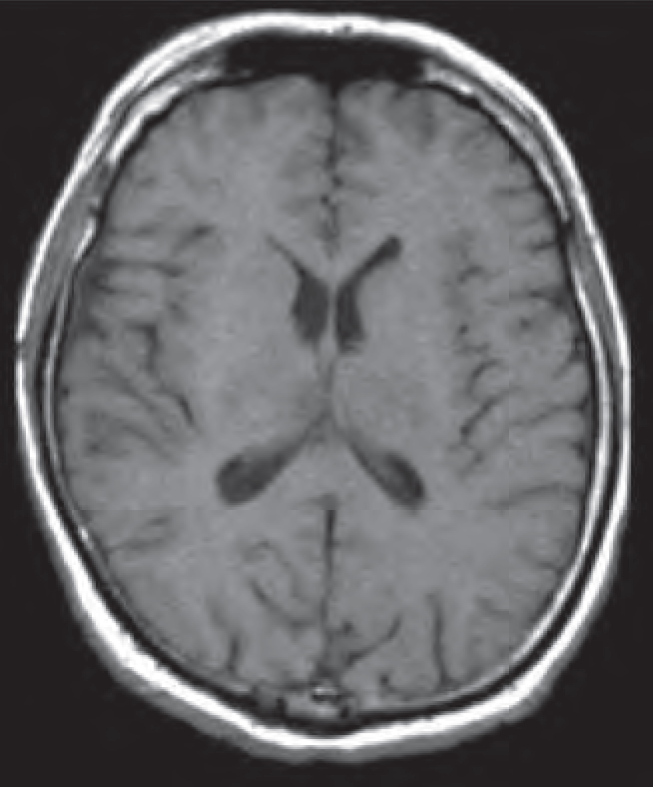
\includegraphics[width=0.3\textwidth]{img/ext/T1Wi.png}}
	\hfill
	\subcaptionbox[T2]{T2 gewichtete Aufnahme ($TR=\SI{3000}{\milli\second}$, $TE=\SI{100}{\milli\second}$)}{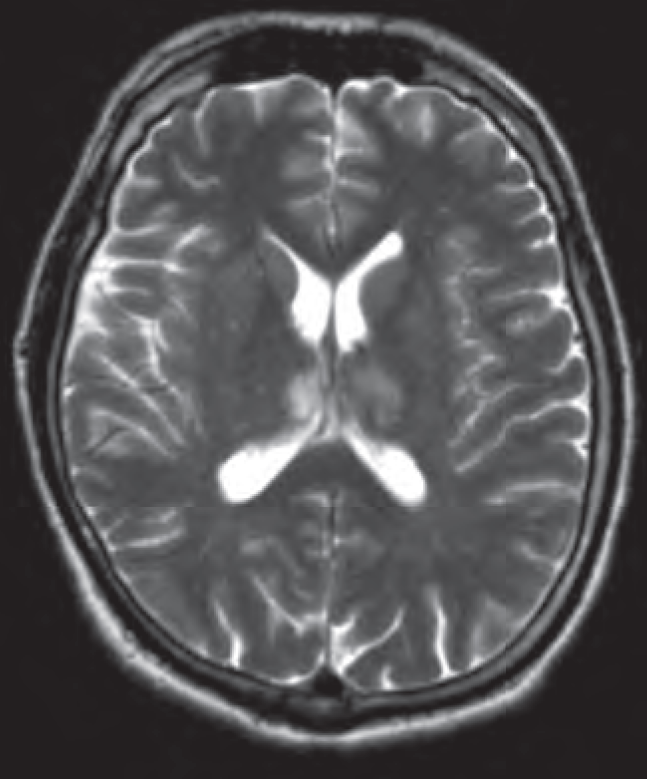
\includegraphics[width=0.3\textwidth]{img/ext/T2Wi.png}}
	\hfill
	\subcaptionbox[PD]{PD gewichtete Aufnahme ($TR=\SI{2400}{\milli\second}$, $TE=\SI{30}{\milli\second}$)}{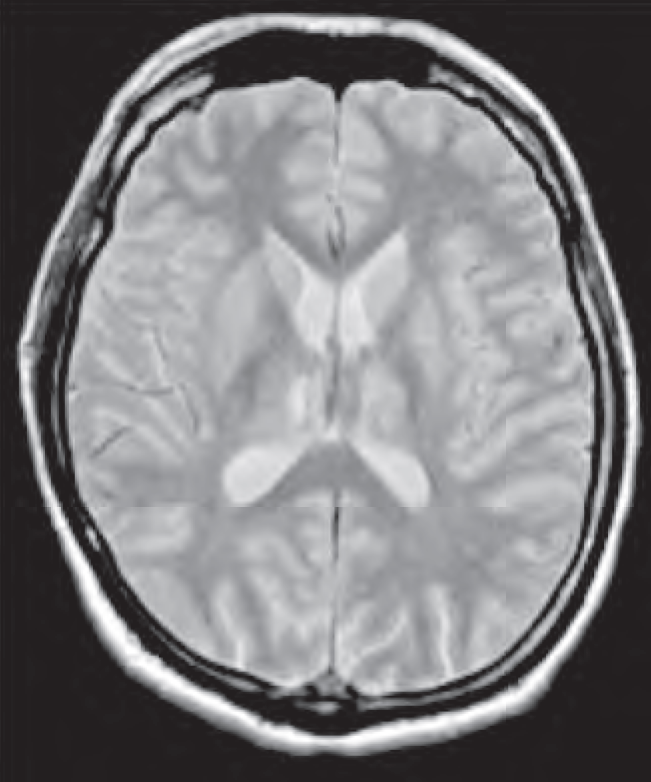
\includegraphics[width=0.3\textwidth]{img/ext/PDWi.png}}
	\caption[Beispiele für unterschiedlich gewichtete Spinecho-Aufnahmen]{Beispiele für verschiedene Gewichtungen eines Schnittbildes durch ein menschliches Gehirn \cite[S.~424ff]{Bushberg2011}}
	\label{fig:BildgewichtungenBsp}
\end{figure}





\subsection{MRT Artefakte}
Zahlreiche Effekte können zu Artefakten in MRT Aufnahmen führen. Welche Artefakte dominieren und ob die Bildqualität wesentlich verschlechtert wird, hängt stark von der Anwendung ab.

Im Wesentliche können die Artefakt-Ursachen in drei Kategorien eingeteilt werden: Gewebeartefakte, Bewegungsartefakte und Artefakte durch die Technik des Tomographen.

\subsubsection{Gewebeartefakte}
Häufige Ursache für Bildartefakte ist die \textit{chemische Verschiebung} ("chemical shift"). Da die Larmorfrequenz eines Kerns von der lokalen magnetischen Feldstärke am Ort des Kerns $B_{lokal}$ und nicht der mittleren Feldstärke über der Probe ($B$) abhängt, kann es durch molekulare Abschirmeffekte zu einer Änderung der Feldstärke $\Delta B$ kommen. Die lokal auf den Kern wirkende Feldstärke ist dann:
\begin{equation}
	B_{lokal}=B+\Delta B
\end{equation}
Empirische Untersuchungen zeigten, dass die Feldabweichung $\Delta B$ proportional zum angelegten Feld ist. Damit ergibt sich $B_{lokal}$ mit dem Abschirmfaktor $\sigma$ zu:
\begin{equation}
	B_{lokal}=B-\sigma B = (1-\sigma)B
\end{equation}
Die Larmorfrequenz ist dann:
\begin{equation}
	\omega = \gamma (1-\sigma)B
\end{equation}

$\sigma$ ist hauptsächlich durch die Verteilung von Elektronen um den Kern und damit von dem molekularen Umfeld abhängig.

Die chemische Verschiebung ist damit nach \cite[S.~24]{Reiser2008} definiert als:
\begin{equation}
\label{eq:chemShift}
	\delta := \frac{\omega-\omega_R}{\omega_0} \cdot 10^6 ~\text{ppm} \approx (\sigma_R-\sigma) \cdot 10^6~\text{ppm}
\end{equation}
mit:
\begin{with}
	\omega   & Larmorfrequenz des betrachteten Kerns\\
	\omega_R & Larmorfrequenz einer Referenzsubstanz\\
	\omega_0 & $=\gamma B_0$ \\
	\sigma   & Abschirmfaktor des betrachteten Kerns \\
	\sigma_R & Abschirmfaktor der Referenz
\end{with}

Die chemische Verschiebung wird, wie in \autoref{eq:chemShift} gezeigt, üblicherweise in "parts per million" (ppm) angegeben.

\subsubsection{Bewegungsartefakte}
Durch Bewegung des untersuchten Lebewesens, sei es durch die willkürliche Muskulatur, oder das Herz bzw. die Atmung, kann es zu Verschiebungen, Verwaschungen oder ähnlichen Bildfehlern in einer Schicht kommen. Außerdem ist es möglich, dass es durch Bewegungen zu Versätzen zwischen aufeinander folgenden Schichten kommt.                       

\subsubsection{Suszeptibilitätsartefakte}
Zu den Suszeptibilitätsartefakte zählen Effekte, die ihre Ursache in Störungen der Magnetfeldhomogenität\footnote{Störungen dieser Art können intrinsisch vorhanden sein, oder durch ferromagnetische Materialien verursacht werden, die durch den zu untersuchenden Körper in das Magnetfeld gebracht werden.}, der RF-Signalkette oder der Rekonstruktion haben.

Durch das Einbringen von ferromagnetischem Material in den Tomograph werden die Feldlinien lokal verzerrt, was einer Änderung der Larmorfrequenzen entspricht. Dadurch entstehen Verzerrungen im Bild oder es erscheinen dunkle Bereiche durch einen Signalverlust in den betreffenden Gebieten.

\subsubsection{Phase Wrapping}
Phase Wrapping, auch als "foldover" oder phase wrap-around bezeichnet führt dazu, dass Strukturen, die außerhalb des gewählten Bildausschnitts liegen, in das Bild hinein gefaltet werden. Der Effekt tritt vor allem durch Aliasing in der Phasenkodierrichtung auf. Eine absolut eingestellte Phase ist nur innerhalb von $2\pi=360\degree$ eindeutig. So kann nicht unterschieden werden, ob eine Phase von z.B. $370\degree$ oder $10\degree$ vorliegt. Die Struktur des rechten Rands mit $\phi=370\degree$ wird daher am Ort von $\phi=10\degree$ abgebildet. Dagegen kann das FOV so vergrößert werden, dass die Orte, die ins Bild gefaltet würden außerhalb vom Körper liegen und daher kein Signal liefern. Auch bietet es sich manchmal an, Frequenzkodier- und Phasenkodierrichtung zu tauschen, da der Effekt in Frequenzkodierrichtung nicht auftaucht, weil dort durch Überabtastung kein Aliasing entsteht \cite{Pusey1988}, \cite{Heiland2008}.

\subsubsection{Geisterbilder bei EPI-Sequenzen}
Durch die Zickzack-Trajektorien bei EPI Sequenzen ist es notwendig, jede zweite akquirierte Zeile zu spiegeln, bevor sie in den k-Raum eingetragen wird. Dabei kann es zu Ausrichtungsfehlern kommen, die sich als Geister im rekonstruierten Bild bemerkbar machen\cite{Ianni2018}.

\subsection{Besonderheiten präklinischer MRT Systeme}
MRTs für die präklinische Bildgebung sind in Bezug auf wirtschaftliche und technische Faktoren auf die Abbildung von Kleintieren optimiert. Da Mäuse, Ratten und andere Nagetiere häufig als Modellorganismen in der Forschung eingesetzt werden, ist das Marktvolumen präklinischer Bildgebungssysteme für diese Tiere am größten. \cite{GBanimalStat} Die Magnetöffnung eines präklinischen MRTs ist daher kleiner als die eines vergleichbaren Gerätes in der Humanmedizin. Während jedoch bei klinischen Tomographen der Durchmesser der Magnetöffnung in etwa den maximalen Patientenabmaßen entspricht, ist die Bohrung eines präklinischen MRTs etwas größer als die Breite der zu untersuchenden Tiere: Da bei den meisten präklinischen MRTs das Gradientensystem und die Empfangsspulen wechselbar ausgeführt sind, muss für diese zusätzlicher Platz in der Bohrung vorgesehen werden. Zur Maximierung der Bildqualität wird der Abstand von Tier zu den Spulensystemen möglichst klein gewählt.

Die Feldstärke des statischen Magnetfeldes ist bei präklinischen MRTs in der Regel höher als bei klinischen: Durch die, im Vergleich zum Menschen, kleineren geometrischen Abmessungen der Tierorgane werden für die präklinische Bildgebung kleinere Voxelgrößen gefordert. Diese führen zu kleineren Signalstärke pro Voxel und damit bei gleichbleibendem Rauschen zu einem reduzierten SNR.

Das relative SNR kann aus der Protonendichte $\rho$, der Stärke des Spinmoments $\mu$, dem Durchmesser der Empfangsspule $d$, dem Voxelvolumen $V_{vox}$ und der Aufnahmezeit $T_{aq}$ abgeschätzt werden \cite[S.~161]{Kiessling2017}:
\begin{equation}
\label{eq:SNR}
	SNR \sim \rho \cdot \mu \cdot B_0 \cdot d^{-1} \cdot V_{vox} \cdot \sqrt{T_{aq}}
\end{equation}
Aus \autoref{eq:SNR} wird ersichtlich, dass bei gleichbleibenden Eigenschaften des Gewebes ($\rho$ und $\mu$) $B_0$ groß gewählt werden muss, wenn $V_{vox}$ klein ist.
Dadurch, dass $B_0$ linear und $T_{aq}$ mit $\sqrt{T_{aq}}$ in die Gleichung eingeht, muss zur Erhaltung eines gegebenen SNRs bei Halbierung der Voxelgröße entweder die Aufnahmezeit vervierfacht werden\footnote{Die Aufnahmezeit ist nach oben durch die maximale Anästhesiezeit der Tiere begrenzt. Für Mäuse beträgt diese etwa eine bis drei Stunden \cite{Kiessling2017}}, oder ein MRT mit doppelter Feldstärke $B_0$ verwendet werden.

Neben den für die Bildqualität entscheidenden Faktoren sind in der präklinischen Bildgebung zusätzlich Handhabungssysteme zur Betäubung, zur konsistenten Positionierung und zum Wärmeerhalt der anästhesierten Tiere im Gerät nötig.

\section{Digitale Signalverarbeitung}
Die RF-Sendesignale und die Spannungen an den Gradientenspulen in der MRT werden von einem sog. Sequenzer digital erzeugt und dann mit einem \gls{dac} in analoge Signale umgesetzt. Die Empfangssignale werden mit einem \gls{adc} wieder in digitale Signale gewandelt.

\subsection{Signale im Frequenzbereich}
Ein zeitdiskretes Signal $x[n]$ entsteht aus einem zeitkontinuierlichen, analogen Signal $x(t)$ durch Abtastung mit der Abtastfrequenz $f_s$. Vor der Abtastung muss der Frequenzgehalt des Signals $x(t)$ durch eine Tiefpassfilterung auf den Bereich $0...\frac{f_s}{2}$ beschränkt werden (Nyquist Theorem).
Für quasi-kontinuierliche Simulationen bei denen sehr hohe Abtastraten verwendet werden, wird oft $x[t]$ statt $x[n]$ geschrieben. Das abgetastete Signal der Länge $N$ ist dann an den diskreten Zeitpunkten
\begin{equation}
	t=0,\,\frac{1}{f_s},\,\frac{2}{f_s},\,...\,,\frac{N-1}{f_s}
\end{equation}
definiert.

Für eine Darstellung im Frequenzbereich wird die \textit{diskrete Fouriertransformation (DFT)} verwendet. Statt DFT wird häufig der Begriff FFT (Fast Fourier Transform) verwendet. Die FFT ist dabei lediglich eine schnelle Implementierung der DFT.
Das Spektrum hat die Frequenzauflösung $df=f_s/N$, die gleiche Länge wie $x[t]$ ($N$) und berechnet sich aus 
\begin{equation}
	X[f]=FFT\{x[n]\}.
\end{equation}
Das Spektrum wird in der Regel auf die Signallänge normiert:
\begin{equation}
X_{norm}[f]=\frac{1}{N} FFT\{x[n]\}.
\end{equation}

Der dazugehörige Frequenzvektor ist:
\begin{equation}
	f=(0,\, df,\, 2df,\, ...\,, f_s-df)-\frac{f_s}{2}
\end{equation}

Das, in der Regel komplexe, Spektrum $X[f]$ kann in Real- und Imaginärteil getrennt dargestellt werden. Üblicher ist jedoch eine Darstellung als einseitiges Amplitudenspektrum. Der, für das einseitige Amplitudenspektrum, nötige Frequenzvektor ist:
\begin{equation}
f=(0,\, df,\, 2df,\, ...\,, \frac{f_s}{2}-df)
\end{equation}
Das normierte, einseitige Amplitudenspektrum ist:
\begin{equation}
X_{norm,abs}[f]=\frac{2}{N} |FFT\{x[n]\}|.
\end{equation}

Beispielspektren für eine Sinus-Funktion sind in \autoref{fig:spectra} dargestellt.

\begin{figure}[H]
	\centering
	\subcaptionbox{$\Re(X[f])$}{\includegraphics[width=0.3\textwidth,height=0.3\textwidth]{plots/dftReal.tikz}}
	\hfill
	\subcaptionbox{$\Im(X[f])$}{\includegraphics[width=0.3\textwidth,height=0.3\textwidth]{plots/dftImag.tikz}}
	\hfill
	\subcaptionbox{$|X[f]|$}{\includegraphics[width=0.3\textwidth,height=0.3\textwidth]{plots/dftAbs.tikz}}
	\caption{Beispielspektren für eine Sinusfunktion der Frequenz \SI{10}{\hertz}; $f_s=\SI{32}{\hertz}, N=16$}
	\label{fig:spectra}
\end{figure}

\subsection{FIR/IIR Filter}
FIR-Filter (eng. finite impulse response filter, Filter mit endlicher Impulsantwort) und IIR-Filter (eng. infinite impulse response filter, Filter mit unendlicher Impulsantwort) sind zwei mögliche diskrete Filterstrukturen. Während sich ein vorgegebener Amplitudenverlauf meist mit einem IIR-Filter geringer Ordnung realisieren lässt, haben FIR-Filter den Vorteil, stets stabil zu sein \cite{Schmidt2014}, \cite{Thyagarajan2019}.

\section{Stochastische Prozesse}
Stochastische Prozesse sind ein hilfreiches Mittel zur Beschreibung von Rauschprozessen.

\subsection{Definition und Kenngrößen}
Ein stochastischer Prozess $x(t,\xi)$ besteht aus einem Zufallsexperiment und einer Zuordnung von Musterfunktionen zu den Elementarereignissen $\xi_\nu$ des Zufallsexperiments \cite[S.~243]{Leon2015}. Der Prozess $x(t,\xi)$ ist eine Funktion von zwei Variablen. Für einen festen Zeitpunkt $t=t_0$ kann $x(t=t_0,\xi)=x_{t_0}(\xi)$ als Zufallsvariable aufgefasst werden. Hingegen wird aus dem Prozess eine gewöhnliche, Zeit-abhängige Funktion, wenn $\xi=\xi_\nu$ konstant gehalten wird. Da in diesem Fall $x(t,\xi=\xi_\nu)=x_{\xi_\nu}(t)$ keinen Zufallscharakter mehr aufweist, ist $x_{\xi_\nu}(t)$ eine deterministische Musterfunktion.

\subsection{Rauschprozesse}
In der Elektronik bezeichnet \textit{Rauschen} eine, zumeist unerwünschte, nicht-\-deterministische Störung eines elektrischen Signals \cite{Heuermann2018}.

Ein Rauschprozess ist als stochastischer Prozess durch sein Leistungsdichtespektrum und die Wahrscheinlichkeitsdichtefunktion seiner Ausgangswerte gegeben.

\section{Phasenrauschen}
Nach \cite{IEEErandom} ist Phasenrauschen definiert als:
\begin{definition}[Phasenrauschen]
	Phasenrauschen beschreibt eine kurzzeitige Abweichungen der Phase von der Nenn-Phase im Frequenzbereich. 
\end{definition}

Für weitere Definitionen wird ein idealer Sinus-Oszillator betrachtet. Sein Ausgangssignal ist durch
\begin{equation}
\label{eq:sinIdeal}
	x_{ideal}(t)=x_0 sin(2\pi \nu_0 t)
\end{equation}
gegeben. Die Phase $\Psi(t)$ ist in diesem Fall linear. Die Momentanfrequenz ist konstant.

Durch Störungen der Amplitude und der Phase des Oszillators ergibt sich:
\begin{equation}
	x_n(t)=[x_0 + e(t)] sin\left(2\pi \nu_0 t + \Phi(t)\right)
\end{equation}

Das Spektrum von $x(t)$ ergibt sich mit der Fourier-Transformation zu:
\begin{equation}
	X(\nu)=\frac{1}{2 i} \left[ \delta(\nu-\nu_0) - \delta(\nu+\nu_0) \right]
\end{equation}

Durch die Einflüsse von $e(t)$ und $\Phi(t)$ verbreitern sich die Dirac-Impulse $\delta(\nu-\nu_0)$ und $\delta(\nu+\nu_0)$.

Phasenrauschen wird nun üblicherweise als Einseitenbandphasenrauschen angegeben. Dies wird mit $\mathscr{L}(f)$ bezeichnet und ist definiert als:
\begin{definition}
	Einseitenbandphasenrauschen ist die Leistung, hervorgerufen durch Phasenfluktuationen, bezogen auf die Gesamtleistung.
\end{definition}[$\mathscr{L}$]
Da der Großteil der Leistung im Träger steckt, kann meist die Gesamtleistung mit der Trägerleistung gleichgesetzt werden. Damit wird $\mathscr{L}$ in Decibel berechnet mit:
\begin{equation}
	\mathscr{L}_{dBc}(f) = P_{n, dBm/Hz} - P_{s, dBm}
\end{equation}

\section{Jitter}

\begin{definition}[Jitter]
	Jitter ist eine (unerwünschte) Störung oder Unsicherheit des Zeitpunkts eines Ereignisses. \cite{Kundert2012}
\end{definition}

Zur Quantifikation von Jitter sind mehrere Metriken gebräuchlich. Die einfachste Metrik ist der \textit{edge-to-edge}-jitter $J_{ee}$. Damit wird die Standardabweichung der Differenzen zwischen einem Ereignis in einem Referenzsignal und einem Testsignal angegeben. Eine Korrelation von Jitter zwischen mehreren Ereignissen kann damit nicht erfasst werden.

Der \textit{k-cycle Jitter}, auch \textit{long term jitter} $J_k$ misst die Variation der Länge von $k$ aufeinander folgenden Zyklen. Für $k=1$ wird diese Metrik auch als \textit{period jitter} bezeichnet.

Der \textit{cycle-to-cycle jitter} $J_{cc}$ misst die Abweichung von zwei aufeinander folgenden Zyklen.

Alle Metriken sind in \autoref{eq:jitterDef} und \autoref{fig:jitterDefs} zusammengefasst.

\begin{subequations}
	\label{eq:jitterDef}
	\begin{align}
	J_{ee}(i)&:=\sqrt{Var\{\delta t_i\}} \\
	J_k(i)&:=\sqrt{Var\{t_{i+k}-t_i\}} \\
	J_{cc}(i)&:=\sqrt{Var\{T_{i+1}-T_i\}}, \quad \text{mit: } T_\alpha=t_{\alpha+1}-t_\alpha
	\end{align}
\end{subequations}

\begin{figure}[H]
	\centering
	\subcaptionbox{Edge-To-Edge-Jitter}{\includegraphics[width=0.55\textwidth]{img/Jitter_edgeToEdge.tikz}}
	\\[4ex]
	\subcaptionbox{$k$-cycle-Jitter}{\includegraphics[width=0.55\textwidth]{img/Jitter_kCycle.tikz}}
	\\[4ex]
	\subcaptionbox{Cycle-To-Cycle-Jitter}{\includegraphics[width=0.55\textwidth]{img/Jitter_cycleToCycle.tikz}}
	\caption[Jitterdefinitionen]{Visualisierung der Jitter-Definitionen in \autoref{eq:jitterDef}; blau: Referenzsignal, grau: gemessenes Signal}
	\label{fig:jitterDefs}
\end{figure}


\subsection{Messverfahren}
Jitter und Phasenrauschen können mit Standard-Messmitteln oder speziellen Analysatoren gemessen werden.

\subsubsection{Im Zeitbereich: Oszilloskop}
Mit einem Oszilloskop kann Jitter direkt visuell abgelesen werden. Auch ein Augendiagramm kann genutzt werden. Damit lassen sich jedoch nur Spitze-zu-Spitze Werte des Jitters bestimmen. Um die Wahrscheinlichkeitsdichte des Jitters zu bestimmen, ist ein Oszilloskop mit Histogrammfunktion notwendig.

\subsubsection{Im Frequenzbereich}
Das Phasenrauschen eines Prüflings (DUT - device under test) kann im Frequenzbereich mit unterschiedlichen Verfahren ausgemessen werden: Die einfachste Vorgehensweise ist das Messen des Spektrums um die Trägerfrequenz mit einem Spektrumanalysator (siehe \autoref{fig:phaseNoiseSA}).
Da hierbei der Träger nicht entfernt wird, ist die Messung hauptsächlich durch den Dynamikumfang des Spektrumanalysators begrenzt. Weiterhin muss für eine sinnvolle Messung des Phasenrauschens nahe der Trägerfrequenz das inhärente Phasenrauschen des Spektrumanalyzers an der betrachteten Offset-Frequenz erheblich kleiner sein, als das des Prüflings. Verfügt der Spektrumanalysator über keinen Phasenrauschmessmodus mit einer Amplitudenrauschunterdrückung, so enthält das gemessene Spektrum neben dem gesuchten Phasenrauschen auch Anteile durch Amplitudenrauschen. Dann muss sichergestellt sein, dass das Amplitudenrauschen gegenüber dem Phasenrauschen so klein ist, dass der Fehler vernachlässigt werden kann. 

\begin{figure}[H]
	\centering
	\resizebox{0.28\textwidth}{!}{\includegraphics[]{img/phaseNoiseMeasurement_SpectrumAnalyzer.tikz}}
	\caption[Spektrumanalysator]{Spectrumanalyzer}
	\label{fig:phaseNoiseSA}
\end{figure}

Ist eine Referenzquelle mit einer Frequenz gleich der Trägerfrequenz des Prüflings verfügbar, kann diese genutzt werden, um das Ausgangssignal des Prüflings auf $f=\SI{0}{\hertz}$ herunter zu mischen. Die spektralen Anteile bei der Summenfrequenz $f=f_{REF}+f_{DUT}$ werden durch einen Tiefpass abgetrennt. Das trägerfreie Phasenrauschsignal kann dann mit dem Spektrumanalyzer gemessen werden.
Gegen Drifts und Phasenrauschen bei sehr kleinen Offsetfrequenzen kann eine PLL verwendet werden, um die Frequenz der Referenzquelle der Trägerfrequenz des Prüflings nachzuführen (\autoref{fig:phaseNoiseMixer}).

\begin{figure}[H]
	\centering
	\resizebox{0.6\textwidth}{!}{\includegraphics[]{img/phaseNoiseMeasurement_Mixer.tikz}}
	\caption[Mischer zur Phasenrauschmessung]{Mischer zur Phasenrauschbestimmung}
	\label{fig:phaseNoiseMixer}
\end{figure}

\section{Bildqualitätsmetriken}
Mit einem MRT erzeugte Schnittbilder der Transversalmagnetisierung von einem Körper sollen helfen, eine Fragestellung in der Diagnostik bzw. Forschung zu beantworten. Neben der Unterscheidung in morphologische und funktionelle Bildgebung, muss auch unterschieden werden, welche Strukturgrößen aufgelöst werden sollen, wie groß der Kontrast benachbarter Gewebetypen sein muss, wie groß das Signal-zu-Rausch-Verhältnis sein darf usw. Außerdem ist für Studien, die über einen längeren Zeitraum durchgeführt werden, die Wiederholgenauigkeit wichtig.

Unabhängig vom Themenfeld der medizinischen (MR)-Bildgebung existieren in der digitalen Bildverarbeitung einige Qualitätsmetriken, mit denen die Qualität eines Bildes geschätzt werden kann, oder die Ähnlichkeit eines Bildes zu einem Referenzbild bewertet werden kann \cite{Wang2006}.

\subsubsection{Qualitätsmetriken ohne Referenz}
Metriken dieses Typs werden auch NR-Metriken (von eng. no reference) genannt. Dabei wird versucht einem Ausgangsbild eines Bildverarbeitungssystems eine Qualitätskennzahl zuzuordnen, ohne, dass das Originalbild vorliegt. Für Menschen ist diese Art der Bildbewertung recht einfach: Durch Vorwissen ist bekannt, dass "gute" Bilder einen hohen Kontrast aufweisen, scharf sind, etc. Aber auch der Inhalt kann in die Bewertung einbezogen werden. So würde ein Mensch ein Bild mit geringer Schärfentiefe nur dann als gut bewerten, wenn die relevanten Bildelemente im Fokus liegen. Für eine automatische Bewertung durch einen Algorithmus muss also auch Vorwissen (eine Heuristik) in Form einer Datenbank mit "guten" Bildern vorliegen, wenn eine inhaltsbezogene Bewertung erreicht werden soll.

Einige Artefakte in Bildern, die durch das Bildaufnahmesystem oder die Verarbeitung eingebracht werden, lassen sich jedoch auch ohne Vorwissen über Analysen im Frequenzbereich oder statistische Methoden detektieren und bewerten \cite[S.~86]{Wang2006}.

Beispiele für NR-Metriken sind der \textit{Naturalness Image Quality Evaluator (NIQE) no-reference image quality score}\cite{Mittal2013} oder die Weiterentwicklung \textit{Perception based Image Quality Evaluator (PIQE) no-reference image quality score}\cite{Venkatanath2015}.

\subsubsection{Qualitätsmetriken mit Referenz}
Bildqualitätsmetriken mit Referenz, auch als FR-Metriken (von eng. full reference) bezeichnet, setzen ein vorhandenes, ideales Originalbild voraus. Diese Metriken fordern in der Regel kein Vorwissen über den Bildinhalt, oder die Klasse von Bildern, die bewertet werden sollen. Statt einer absoluten Qualitätskennzahl wird ein Ähnlichkeitsmaß zwischen untersuchtem Bild und Referenzbild bestimmt \cite[S.~43]{Wang2006}.

Eine einfache Möglichkeit für eine FR-Metrik ist die (zweidimensionale) \textit{mittlere quadratische Abweichung}, auch MSE (für eng. \textit{mean squared error}) genannt. Definiert ist der MSE zwischen einem $N \times M$ großen Bild $X$ und einem ebenso großen Referenzbild $R$ als \cite{Tan2013}:

\begin{equation}
	MSE_R(X)=\frac{1}{M N} \sum_{n=1}^{N} \sum_{m=1}^{M} [X(n,m) - R(n,m)]^2
\end{equation}

Aus dem MSE und dem Dynamikbereich beider Bilder $L$ (für ein 8-bit Bild ergibt sich $L=255-0=255$) kann das \textit{peak signal-to-noise ratio\footnote{Eine deutsche Bezeichnung ist nicht üblich.}} (PSNR) berechnet werden. Das PSNR ist definiert als \cite{Bondzulic2016}:
\begin{equation}
	PSNR_R(X)= 10\: log_{10}\left(\frac{L^2}{MSE_R(X)}\right) = 20\: log_{10}(L) - 10\: log_{10}(MSE_R(X))
\end{equation}

Eine komplexere Metrik ist die \textit{Strukturelle Ähnlichkeit}, \textit{SSIM} (von eng. \textit{structural similarity}). Sie wurde 2004 in \cite{Wang2004} als Verbesserung der Metriken MSE bzw. PSNR vorgeschlagen. Die SSIM zwischen $X$ und dem Referenzbild $R$ ist definiert als:
\begin{equation}
	SSIM_R'(X)=[l(X,R)]^\alpha\cdot[c(X,R)]^\beta\cdot[s(X,R)]^\gamma
\end{equation}
mit:
\begin{with}
	l(X,R) & Luminanz-Ähnlichkeit\\
	c(X,R) & Kontrast-Ähnlichkeit\\
	s(X,R) & Struktur-Ähnlichkeit\\
	\alpha,\beta,\gamma & Gewichtungsfaktoren \\
\end{with}

Die Luminanz-, Kontrast- und Strukturähnlichkeiten sind dabei wie folgt definiert:

\begin{subequations}
	\begin{align}
	l(X,R) & = \frac{2\mu_X\mu_R+c_1}{\mu_X^2+\mu_R^2+c_1}\\
	c(X,R) & = \frac{2\sigma_X\sigma_R+c_2}{\sigma_X^2+\sigma_R^2+c_2}\\
	s(X,R) & = \frac{\sigma_{XR}+c_3}{\sigma_X\sigma_R+c_3}
	\end{align}
\end{subequations}
mit:
\begin{with}
	\mu_X,\mu_R & Mittelwerte von $X$ bzw. $R$\\
	\sigma_X,\sigma_R & Standardabweichungen von $X$ bzw. $R$\\
	\sigma_{XR} & Kovarianz von $X$ und $R$\\
	c_1=(k_1L)^2 & "Stabilisierungsvariable"\\
	c_2=(k_2L)^2 & "Stabilisierungsvariable"\\
	L & Dynamikumfang der Bilder (255 bei zwei 8-bit Bildern)
\end{with}
$k_1$ und $k_2$ sind wählbare Parameter mit $k_1,k_2 \ll 1$\footnote{Standardwerte in der SSIM Implementierung \texttt{ssim()} der MATLAB Image Processing Toolbox sind: $k_1=0.01$ und $k_2=0.03$}.

In der Regel wird $c_3=c_2/2$ gewählt und $\alpha=\beta=\gamma=1$ gesetzt. Damit ergibt sich:
\begin{equation}
	SSIM_R(X) = \frac{\left(2\mu_X\mu_R+c_1\right)\left(2\sigma_{XR}+c_2\right)}{\left(\mu_X^2+\mu_R^2+c_1\right)\left(\sigma_X^2+\sigma_R^2+c_2\right)}
\end{equation}

Im Gegensatz zu MSE und PSNR, die absolute Abweichungen bewerten, ist die Schätzung bei SSIM mehr an der Wahrnehmung des Menschen orientiert. Eine Degradation des Bildes wird mit einer Änderung an Strukturinformationen gleichgesetzt. Neben der reinen Strukturmetrik fließen zusätzlich Bewertungen der Phänomene "Helligkeitsmaskierung" und "Kontrastmaskierung" in die SSIM Metrik ein. Diese Begriffe aus der Wahrnehmungspsychologie beschreiben eine Abnahme der Auffälligkeit von Strukturänderungen in hellen Bildbereichen bzw. Bereichen mit starken Kontrasten \cite{Wang2004}.

Abwandlungen und Erweiterungen der SSIM sind neben der \textit{M-SSIM}, bei der lediglich eine Mittelung/Glättung vorgenommen wird, zum Beispiel:

\begin{itemize}
	\item \textbf{CW-SSIM\cite{Gao2011}:} Bei der \textit{Complex Wavelet Structural Similarity} wird die SSIM dahingehend verbessert, dass sich einige Bildstörungen, die nur die Phase der komplexen Wavelet-Koeffizienten eines Bildes, nicht aber die Struktur ändern, weniger stark auf die Metrik auswirken.
	\item \textbf{MS-SSIM\cite{Wang2003}:} Die \textit{Multi Scale Structural Similarity} versucht der menschlichen Wahrnehmung noch näher zu kommen durch die Nutzung von unterschiedlich feinen Abtastungen der zu vergleichenden Bilder.
	\item \textbf{IW-SSIM\cite{Wang2011}:} \textit{Information Content Weighted Structural Similarity Measure} ist eine SSIM Variante, in der zusätzlich Konzepte aus der Informationstheorie für die Erzeugung von Gewichtungsfaktoren genutzt werden.
\end{itemize}

Für die in \autoref{fig:metrikenTest} gezeigten Bilder sind die oben erläuterten Metriken in \autoref{tab:metriken} aufgeführt.

\begin{figure}[H]
	\centering
	\subcaptionbox{Originalbild}{
\includegraphics[width=0.45\textwidth]{img/metrics/brukerNorm.png}}
	\\[4ex]
	\subcaptionbox{Weichzeichnung mit einem 15x15 Gauß-Filter}{
\includegraphics[width=0.45\textwidth]{img/metrics/brukerBlur15.png}}
	\hfill
	\subcaptionbox{weißes Rauschen mit $\sigma=10$}{
\includegraphics[width=0.45\textwidth]{img/metrics/brukerNoise.png}}
	\\[4ex]
	\subcaptionbox{Verschiebung um $\vec{d}(x,y)=(-10,-10)$}{
\includegraphics[width=0.45\textwidth]{img/metrics/brukerShift10.png}}
	\hfill
	\subcaptionbox{Verschiebung um $\vec{d}(x,y)=(-20,-20)$}{
\includegraphics[width=0.45\textwidth]{img/metrics/brukerShift20.png}}
	\caption[Testbilder für Bildqualitätsmetriken]{Testbilder für den Vergleich einiger Bildqualitätsmetriken}
	\label{fig:metrikenTest}
\end{figure}

\begin{table}[H]
	\centering
	\caption[Vergleich Bildqualitätsmetriken]{Vergleich einiger Bildqualitätsmetriken mit den Testbildern in \autoref{fig:metrikenTest}}
	\label{tab:metriken}
	\begin{tabular}{lSSSSS}
		\toprule
		\textbf{Metrik} & \textbf{(b)} & \textbf{(c)} & \textbf{(d)} & \textbf{(e)} & \textbf{(a), Referenz} \\
		\midrule
		SSIM    & 0.825 & 0.0331 & 0.871 & 0.831 & 1 \\
		CW-SSIM & 0.999 & 0.981  & 0.987 & 0.951 & 1 \\
		M-SSIM  & 0.836 & 0.048  & 0.882 & 0.839 & 1 \\
		MS-SSIM & 0.958 & 0.401  & 0.815 & 0.721 & 1 \\
		IW-SSIM & 0.617 & 0.435  & 0.078 & 0.067 & 1 \\
		& & & & & \\
		MSE     & 397     & 1971     & 3506    & 6205    & 0 \\
		PSNR    & -25.98  & -32.95   & -35.45  & -37.93  &  \\
		NIQE    & 11.52   & 23.80    & 12.48   & 12.55   & 12.58 \\
		\bottomrule
	\end{tabular}
\end{table}

Exemplarisch sind die verschiedenen SSIM Qualitätsmetriken in \autoref{fig:vergleichSSIM} dargestellt.

\begin{figure}[H]
	\centering
	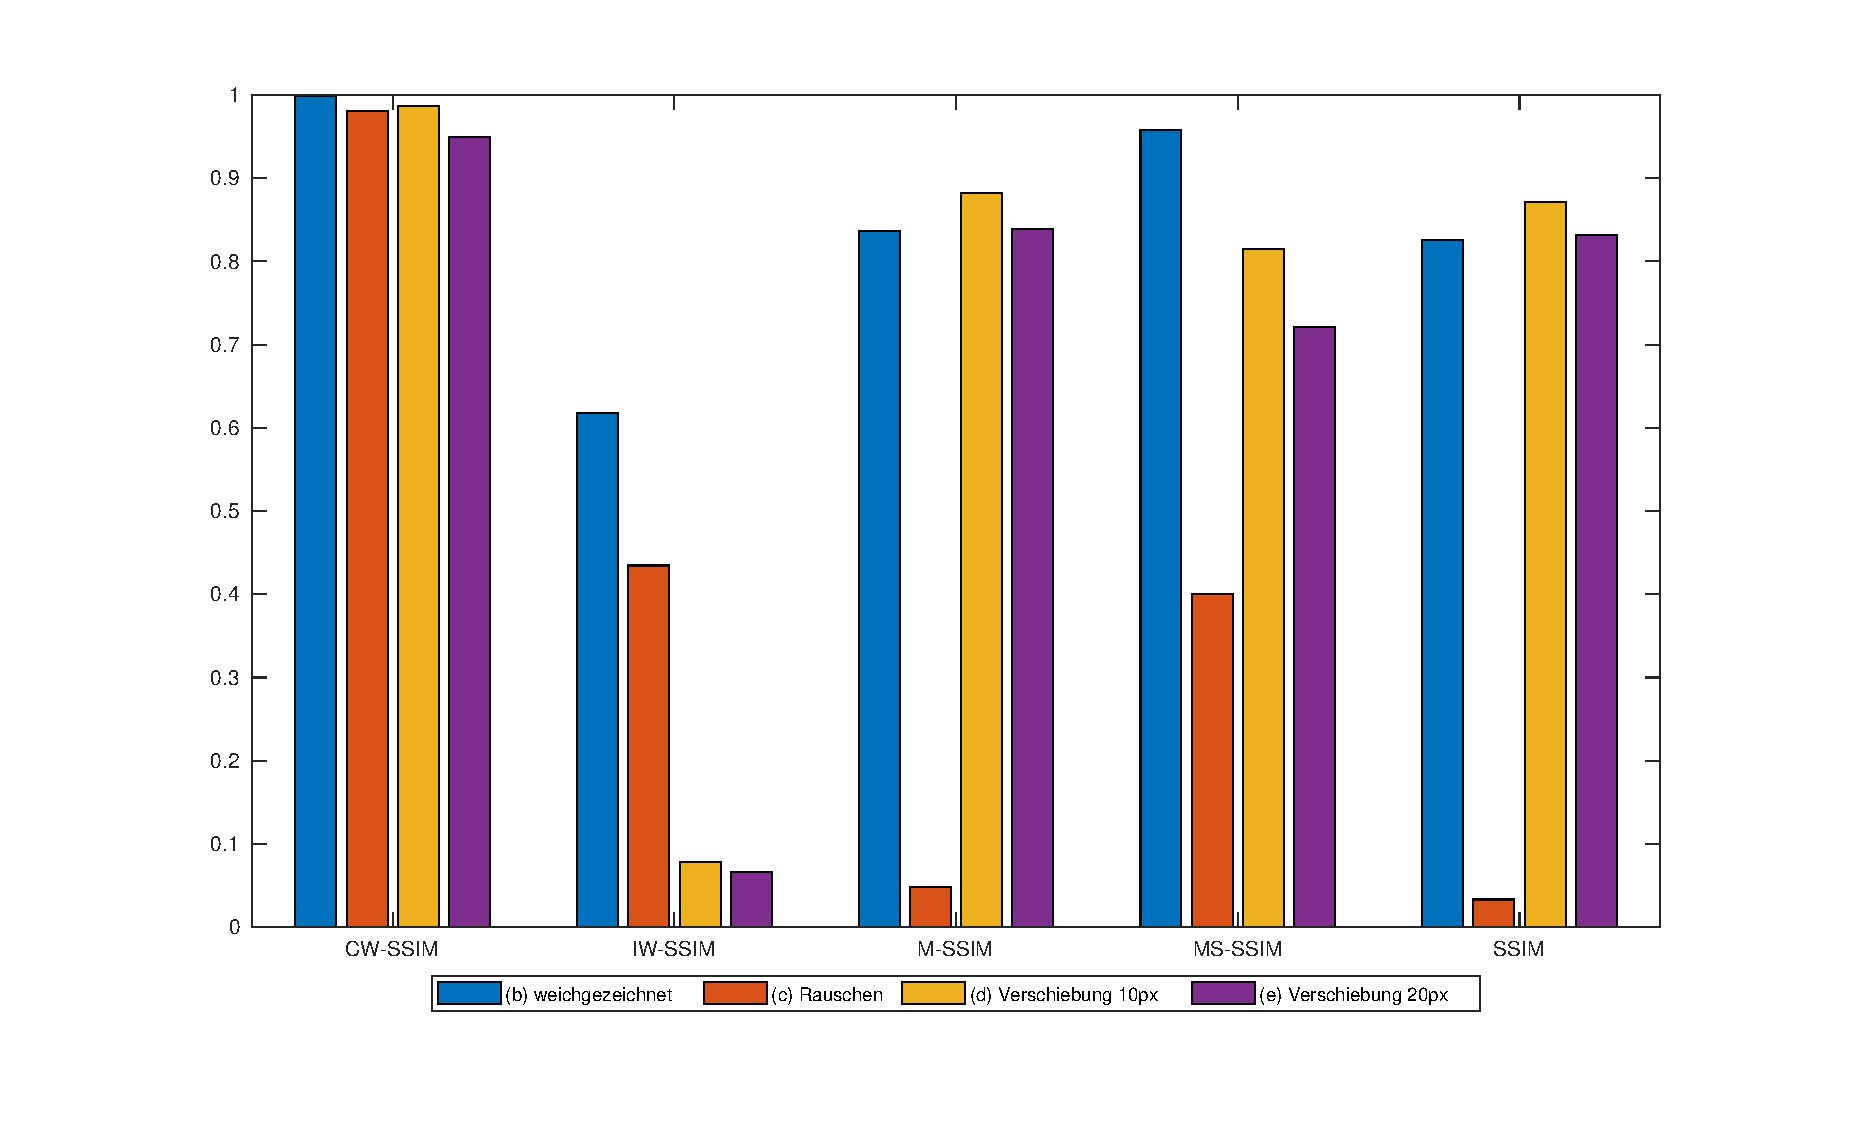
\includegraphics[width=\textwidth]{img/metrics/ssimComp.eps}
	\caption[Vergleich verschiedener SSIM Varianten]{Vergleich verschiedener SSIM Varianten, Daten aus \autoref{tab:metriken}}
	\label{fig:vergleichSSIM}
\end{figure}

Für die Qualitätsbewertung in der medizinischen Bildgebung sind SSIM und die Derivate MS-SSIM, CW-SSIM, etc. etabliert (\cite{Punga2014}, \cite{VenkatNarayanaRao2013}) und zeigen in der Regel eine höhere Robustheit gegen Translationen als MSE oder PSNR.















